\documentclass{beamer}

\usepackage[utf8]{inputenc}
\usepackage{amsmath}
\usepackage{graphicx}
\usepackage{pdflscape}
\usepackage{geometry}
\usepackage{xcolor}
\usepackage{bookmark}
\usepackage[numbers]{natbib}

%\setbeameroption{hide notes} % Only slides
%\setbeameroption{show only notes} % Only notes
\setbeameroption{show notes on second screen=right} % Both
\setbeamertemplate{footline}[frame number]

\setbeamercolor{note page}{bg=white,fg=black}
\setbeamerfont{note page}{size=\footnotesize}
\setbeamertemplate{caption}[numbered]
\setbeamercolor{frametitle}{bg=blue, fg=white}
\setbeamercolor{title}{bg=blue, fg=white}

\title{\textbf{\textsf{Neural mechanisms in processing of Emotion in Real and Virtual faces}}}
\subtitle{\textsf{Using functional-near infrared spectroscopy (fNIRS)}}
\author{Dylan Rapanan}
\newcommand{\supervisor}{Supervised by: Dr. Steven Livingstone and Dr. Bobby Stojanoski}
\date{\today}

\begin{document}

\begin{frame}
    \titlepage
    \vfill
    \begin{center}
        \text{\supervisor}
    \end{center}
    \vfill
    \centering
    \begin{columns}
        \begin{column}{0.35\textwidth}
            
\includegraphics[width=1\textwidth]{C:/Users/super/OneDrive - Ontario Tech University/fNIRS_Emotions/plots/figures/OntarioTech Logo.png}
        \end{column}
        \begin{column}{0.35\textwidth}
            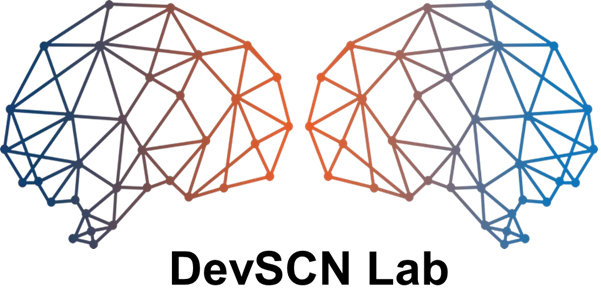
\includegraphics[width=1\textwidth]{C:/Users/super/OneDrive - Ontario Tech University/fNIRS_Emotions/plots/figures/DevSCN Lab.png}
        \end{column}
        \begin{column}{0.35\textwidth}
            
\includegraphics[width=1\textwidth]{C:/Users/super/OneDrive - Ontario Tech University/fNIRS_Emotions/plots/figures/ADSL.png}
        \end{column}
    \end{columns}
   \note[frame]{
        \begin{itemize}
            \item Hello everyone, my name is Dylan Rapanan, and I am a Master's student in Computer Science at Ontario Tech University and I am co-supervised by Dr. Steven Livingstone and Dr. Bobby Stojanoski. 
            \item Today, I will be presenting my research on the neural mechanisms involved in processing emotion in real and virtual faces using functional near-infrared spectroscopy (fNIRS).
        \end{itemize}
    }
\end{frame}

\begin{frame}
    \frametitle{Introduction}
    \framesubtitle{Background: The Importance of Faces and Emotional Expressions}
    \begin{columns}[c]
        \begin{column}{0.3\textwidth}
            \centering
            \includegraphics[width=0.5\textwidth]{C:/Users/super/OneDrive - Ontario Tech University/fNIRS_Emotions/RADIATE Color Faces/RADIATE_COLOR_8/HM10/HM10_HC.png}
        \end{column}
        \begin{column}{0.3\textwidth}
            \centering
            \includegraphics[width=0.5\textwidth]{C:/Users/super/OneDrive - Ontario Tech University/fNIRS_Emotions/RADIATE Color Faces/RADIATE_COLOR_1/AF10/AF10_HC.png}
        \end{column}
    \end{columns}
    \begin{itemize}
        \item Our brains are evolutionarily primed to process faces, as they are crucial for social interactions.
        \item A central aspect of facial perception is emotional expressions, which underpins our interactions as social beings.
        \item It is currently unclear how the brain processes emotional expressions, despite much research. \cite{kawasaki_processing_2012}
        \item Early models of facial perception proposed modular processing: face identity was linked to the fusiform face area (FFA) \cite{kawasaki_processing_2012}, while emotional expressions were associated with limbic structures like the amygdala. \cite{sato_amygdala_2004}
    \end{itemize}
    \note[frame]{
        \begin{itemize}
            \item Our brains are evolutionarily primed to process faces, as they are crucial for social interactions.
            \item A central aspect of facial perception is emotional expressions, which underpins our interactions as social beings.
            \item It is currently unclear how the brain processes emotional expressions, despite much research.
            \item Early models of facial perception proposed that face identity was linked to the fusiform face area (FFA), while emotional expressions were associated with limbic structures like the amygdala.
            \item This is the idea that there are specific locations or areas in the brain that are responsible for processing faces and emotions. 
        \end{itemize}
    }
\end{frame}

\begin{frame}
    \frametitle{Introduction}
    \framesubtitle{Background: The Shift to Virtual Environments}
    \begin{columns}[c]
        \begin{column}{0.3\textwidth}
            \centering
            \includegraphics[width=0.5\textwidth]{C:/Users/super/OneDrive - Ontario Tech University/fNIRS_Emotions/UIBVFED_cropped/JOY/Dave_SmilingClosedMouth.png}
        \end{column}
        \begin{column}{0.3\textwidth}
            \centering
            \includegraphics[width=0.5\textwidth]{C:/Users/super/OneDrive - Ontario Tech University/fNIRS_Emotions/UIBVFED_cropped/JOY/Alicia_SmilingClosedMouth.png}
        \end{column}
    \end{columns}
    \begin{itemize}
        \item As humans spend increasing time in digital and virtual environments, we interact more and more with computer-generated/avatar faces in our lives. 
        \item While real-face emotion processing has been studied extensively, the neural mechanisms for perceiving and responding to virtual faces remain poorly understood. \cite{de_borst_is_2015}
        \item Recent evidence suggests face and emotion processing recruit distributed brain networks rather than isolated “face areas,” pointing to a need for network-level investigation. \cite{lindquist_brain_2012}
    \end{itemize}
    \note[frame]{
        \begin{itemize}
            \item So contrast the faces we just saw with these virtual faces here, do you think the brain processes these faces in the exact same way as real faces?
            \item You see, as humans spend more time in digital and virtual environments, we interact more with computer-generated or avatar faces.
            \item And while real-face emotion processing has been studied extensively, the neural mechanisms for perceiving and responding to virtual faces remain poorly understood. 
            \item As well, recent evidence suggests that face and emotion processing recruit distributed brain networks rather than isolated “face areas,” which points to a need for network-level investigation.
            \item This means that instead of just one area of the brain being responsible for processing faces and emotions, there are multiple areas that work together to do this.
            \item So let's lay out what exactly we want to find out in this study.
        \end{itemize}
    }
\end{frame}

\begin{frame}
    \frametitle{Introduction}
    \framesubtitle{Research Objectives/Hypotheses}
    \begin{itemize}
        \item \textbf{Objective:} Identify distinct patterns of brain activity that represent processing of different emotions on real and virtual faces.
        \item \textbf{Hypotheses:}
             \begin{enumerate}
                    \item $H_1$: Differential activity between real and virtual faces. \\ 
                    \item $H_2$: Differential activity across different emotions (anger, disgust, fear, happiness, sadness, surprise, neutral). \\ 
             \end{enumerate}
    \end{itemize}
    \note[frame]{
        \begin{itemize}
            \item The objective of this research is to identify distinct patterns of brain activity that represent the processing of different emotions on real and virtual faces.
            \item We have two hypotheses: first, we expect to see differences in brain activity between real and virtual faces, and second, we expect to see differences in brain activity across different emotions, such as anger, disgust, fear, happiness, sadness, surprise, and neutral.
            \item These are the 7 basic emotions that we are looking at in this study.
        \end{itemize}
    }
\end{frame}

\begin{frame}
    \frametitle{Methodology}
    \framesubtitle{Participants}
    \begin{itemize}
        \small
        \item Participants were recruited from the Ontario Tech University SONA system and were compensated with course credit.
        \item 87 participants completed the experiment, but only 52 participants were included after excluding those with poor data quality.
        \item We used thresholds common in fNIRS research such as the Scalp Coupling Index (SCI) to determine the quality of the data.
        \item The 52 participants ranged in age from 17-51 years old, with a mean age of 22 years, and 39/52 were female. 
    \end{itemize}
    \note[frame]{
        \begin{itemize}
            \item Participants were recruited from the Ontario Tech University SONA system and were compensated with course credit for their participation.
            \item A total number of 87 participants completed the experiment, but only 52 participants were included in the fNIRS analysis after excluding those with poor data quality.
            \item We used thresholds common in fNIRS research such as the Scalp Coupling Index (SCI) to determine the quality of the data.
            \item In terms of demographics, the 52 participants ranged in age from 17-51 years old, with a mean age of 22 years, and 39 out of 52 were female. 
        \end{itemize}
    }
\end{frame}

\begin{frame}
    \frametitle{Methodology}
    \framesubtitle{Functional Near-Infrared Spectroscopy (fNIRS)}
    \begin{itemize}
        \item \textbf{Functional near-infrared spectroscopy (fNIRS)} is a non-invasive tool that tracks changes in blood oxygen levels in the brain as an indirect measure of neural activity.
    \end{itemize}
    \begin{figure}
        \centering
        \begin{minipage}{0.3\textwidth}
            \centering
            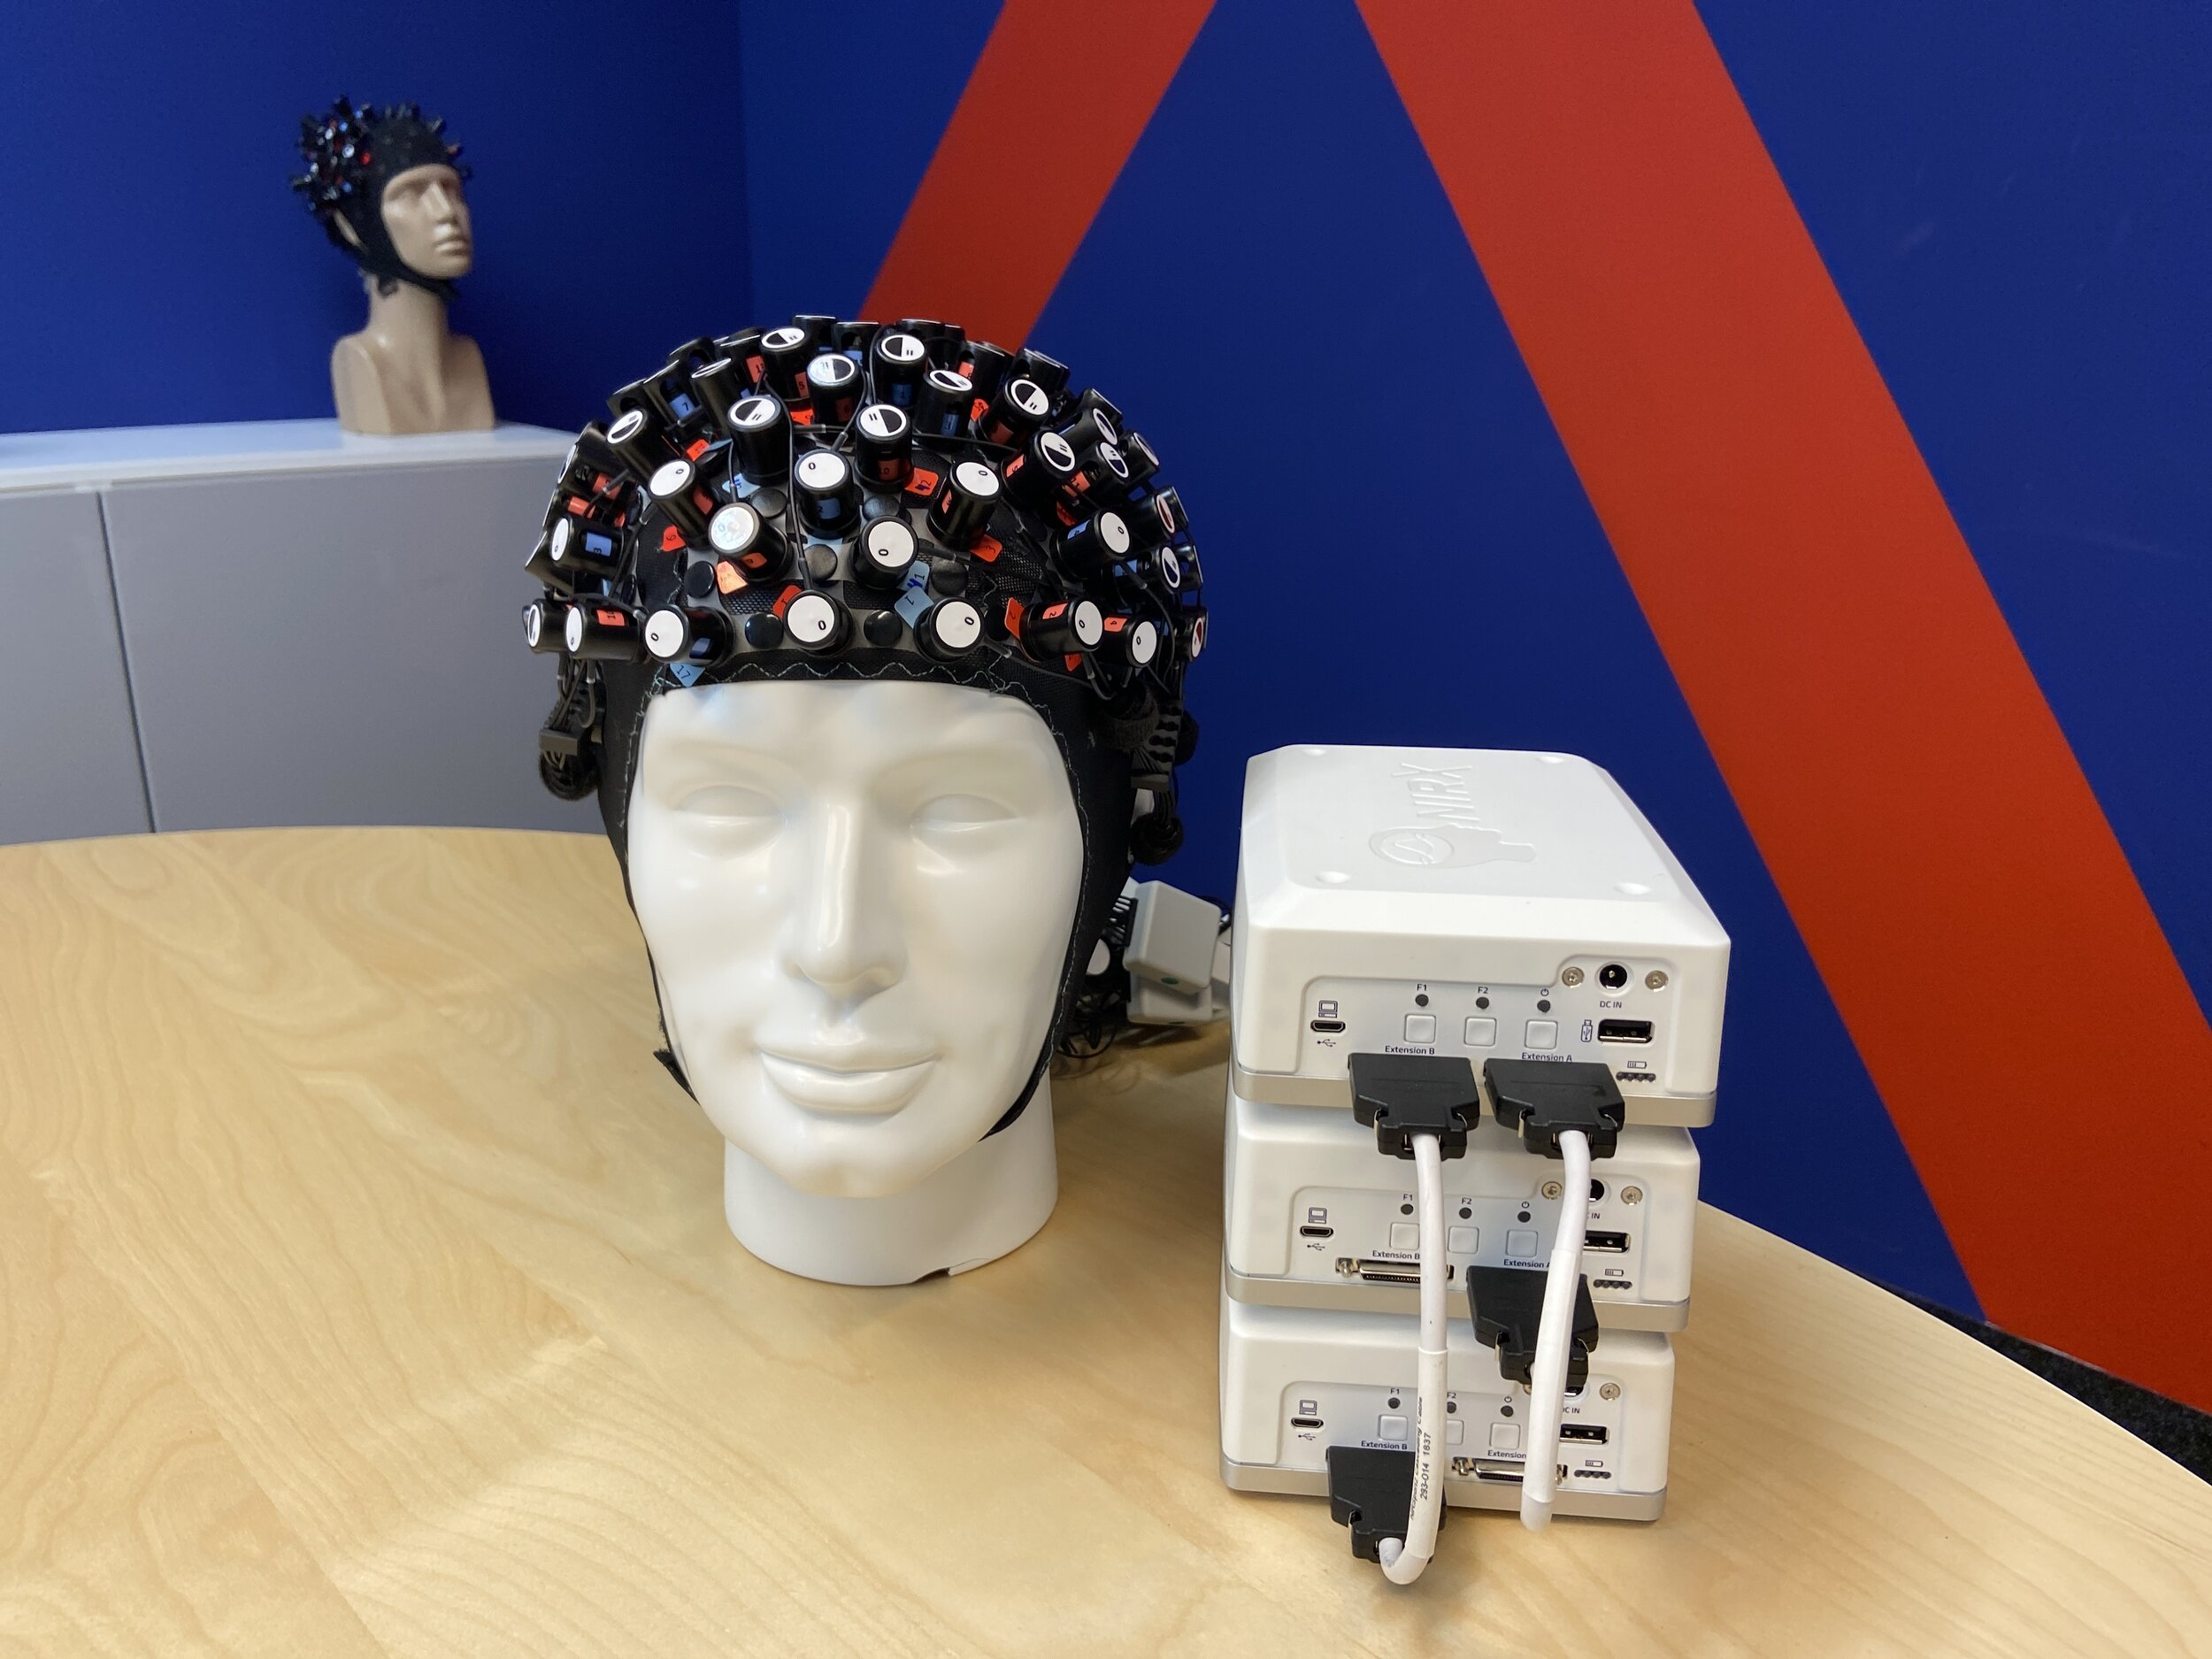
\includegraphics[width=1\textwidth]{C:/Users/super/OneDrive - Ontario Tech University/fNIRS_Emotions/plots/figures/fNIRS picture.jpg}
        \end{minipage}
        \hfill
        \begin{minipage}{0.65\textwidth}
            \centering
            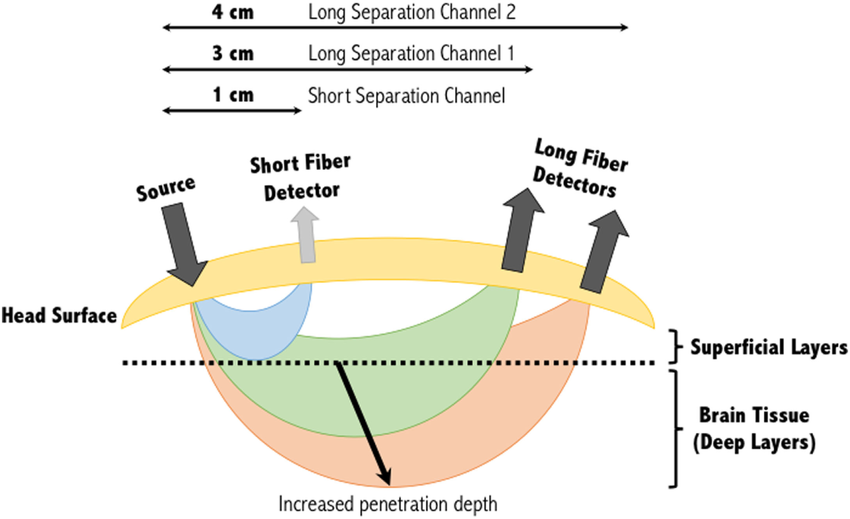
\includegraphics[width=1\textwidth]{C:/Users/super/OneDrive - Ontario Tech University/fNIRS_Emotions/plots/figures/Channel Diagram.png}
        \end{minipage}
    \end{figure}
    \note[frame]{
        \begin{itemize}
            \item In order to quantify differences in brain activity, we need a tool called functional near-infrared spectroscopy (fNIRS).
            \item So what is fNIRS? fNIRS is a non-invasive tool that tracks changes in blood oxygen levels in the brain as an indirect measure of neural activity.
            \item How does fNIRS work? It works by shining near-infrared light into the scalp and measuring how much light is absorbed and scattered by brain tissue.
            \item There are tiny light sources called emitters and light sensors called detectors that are placed on the scalp, the emitters send light into the head, and the detectors record the back-scattered light that emerges.
            \item fNIRS estimates shifts in blood oxygenation, which provides insights into which brain areas are active.
        \end{itemize}
    }
\end{frame}

\begin{frame}
    \frametitle{Methodology}
    \framesubtitle{fNIRS Data Acquisition}
    \begin{figure}
        \centering
        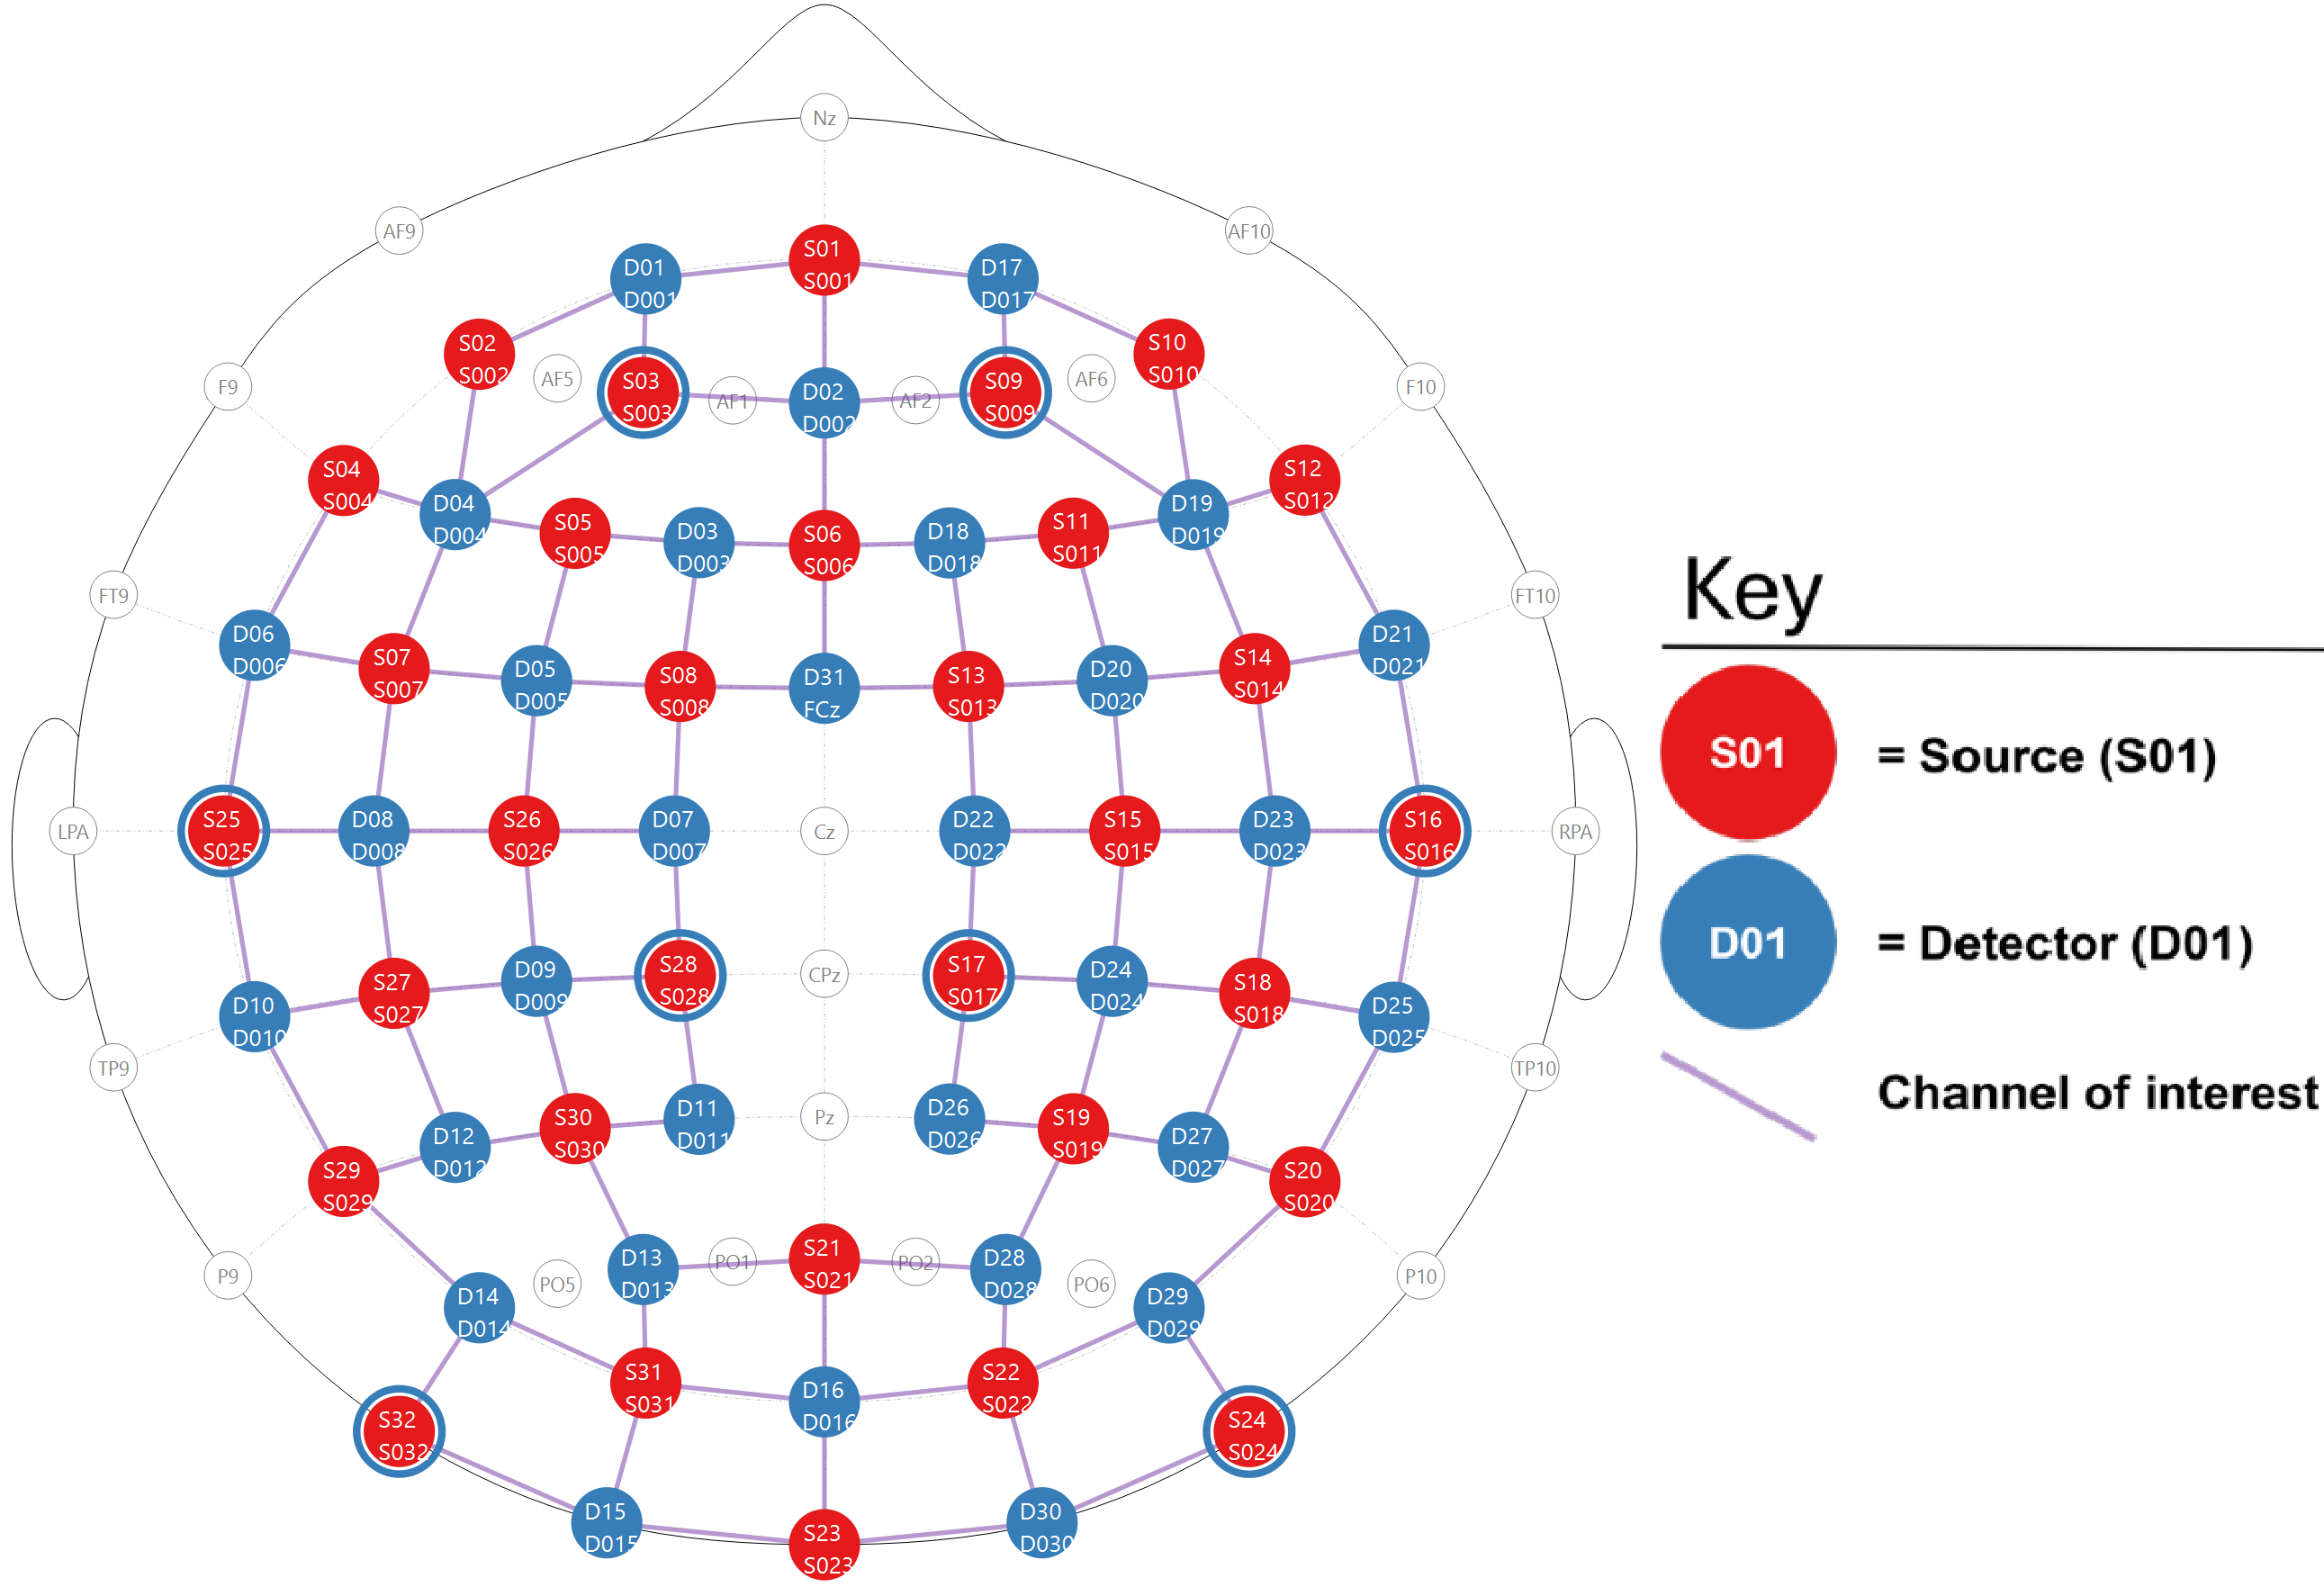
\includegraphics[width=0.7\textwidth]{C:/Users/super/OneDrive - Ontario Tech University/fNIRS_Emotions/plots/figures/Montage.png}
    \end{figure}
    \begin{itemize}
        \small
        \item Montage of fNIRS cap, which shows the placement of the optodes on the scalp.
        \item Each neighboring pair of source (red) and detector (blue) optode is referred to as a channel (purple line), resulting in 103 channels.
    \end{itemize}
    \note[frame]{
        \begin{itemize}
            \item So here is the montage of fNIRS cap, which shows the placement of the optodes on the scalp.
            \item Each neighboring pair of source (red) and detector (blue) optode is referred to as a channel (purple line), this results in 103 channels in total.
            \item We aimed to cover a maximal area of the brain with this montage, as facial and emotional processing is distributed across the cortex.
        \end{itemize}
    }
\end{frame}

\begin{frame}
    \frametitle{Methodology}
    \framesubtitle{Design and Procedure}
    \begin{figure}
        \centering
        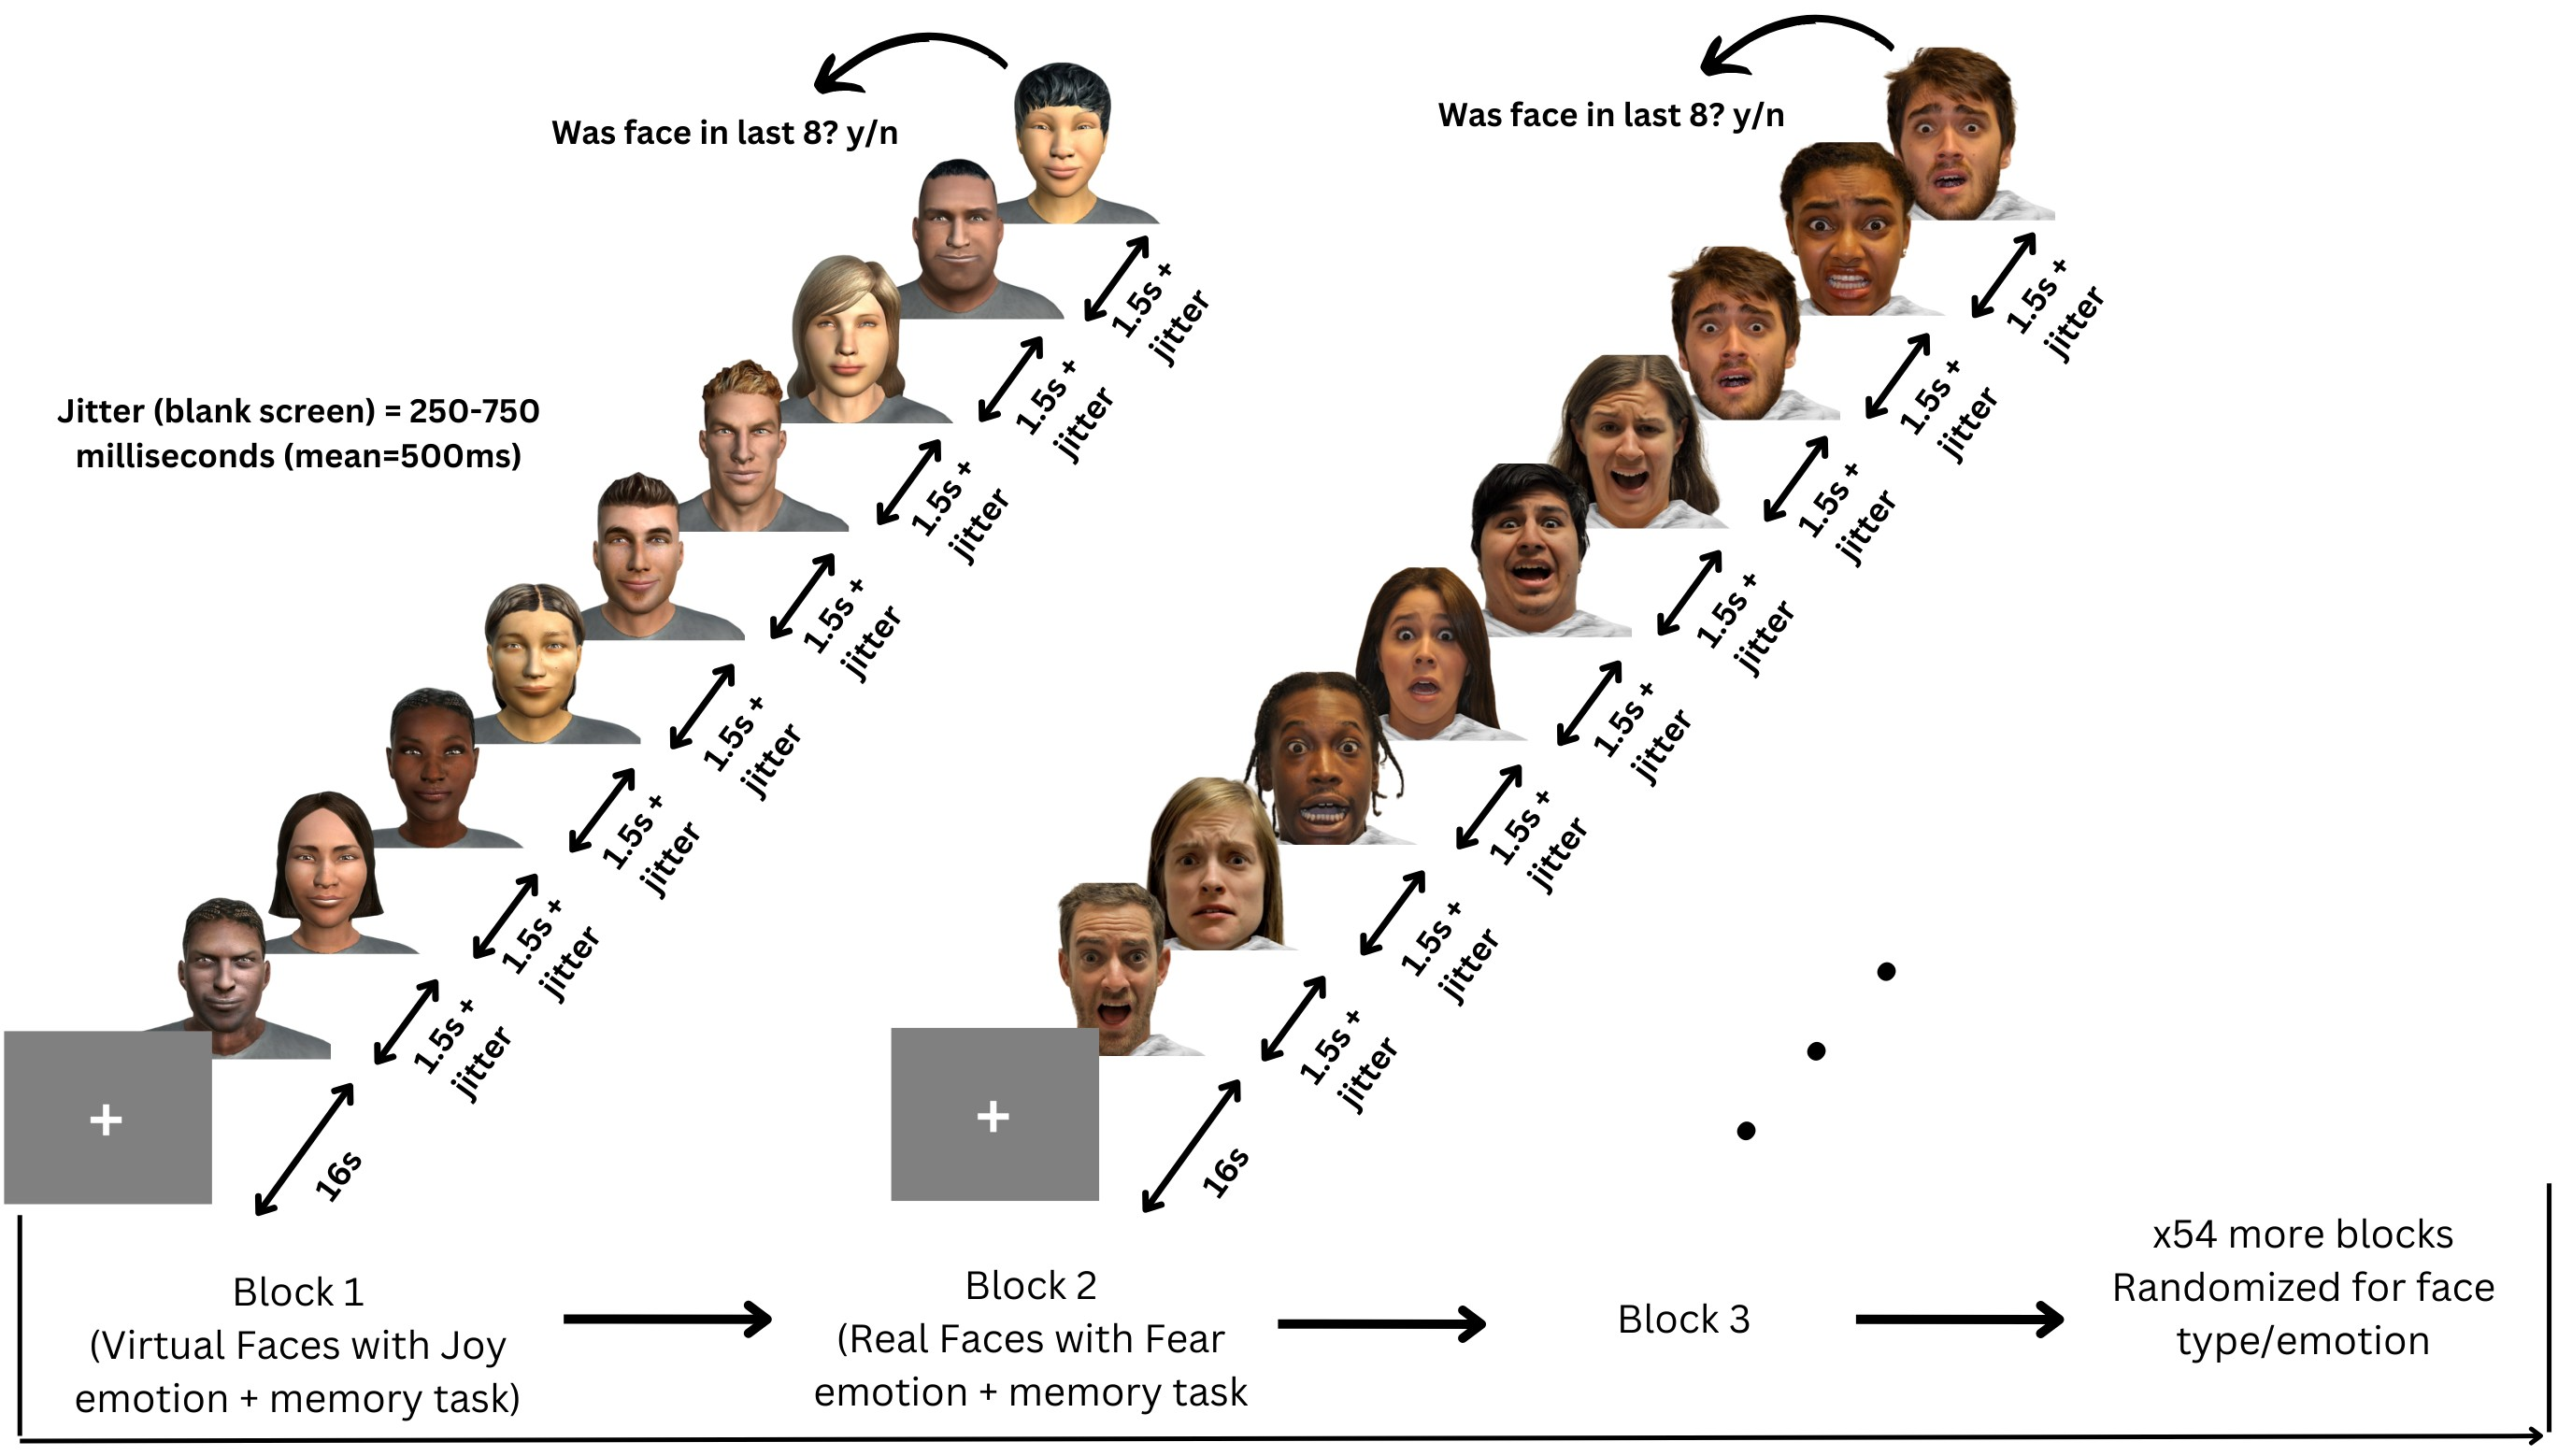
\includegraphics[width=0.8\textwidth]{C:/Users/super/OneDrive - Ontario Tech University/fNIRS_Emotions/plots/figures/Paradigm.jpg}
    \end{figure}
    \begin{itemize}
        \small
        \item Participants viewed 56 blocks of 8 faces, each block being either all real or all virtual faces.
        \item Every face in a block displayed the same emotional expression, one of: anger, disgust, fear, happiness, sadness, surprise, neutral. 
        \item \textbf{Memory task:} Participants had to indicate whether the 9th face was present in the previous 8 faces by answering "yes" or "no".
    \end{itemize}
    \note[frame]{
        \begin{itemize}
            \item So here was the experiment: participants viewed 56 blocks of faces, with each block containing 8 faces of the same emotion (e.g., joy, fear) and type (real or virtual). 
            \item The faces were shown one at a time for 1.5 seconds each, with short random jitters of about half a second between them.
            \item After the 8 faces were shown, participants had to indicate whether the 9th face was present in the previous 8 faces by answering "yes" or "no" within 7 seconds, this was the \textbf{memory task} they had to do for the main purpose of keeping them engaged and focused on the faces. 
            \item As for the actual faces that were shown, we selected 20 models—10 from the RADIATE dataset of real people and 10 from the UIBVFED dataset of virtual characters—ensuring a balanced mix of gender and ethnic diversity. 
            \item Each model was carefully matched across datasets by facial features, and emotional expression. 
        \end{itemize}
    }
\end{frame}

\begin{frame}
    \frametitle{Analyses}
    \framesubtitle{Preprocessing Steps}
    \begin{figure}
        \centering
        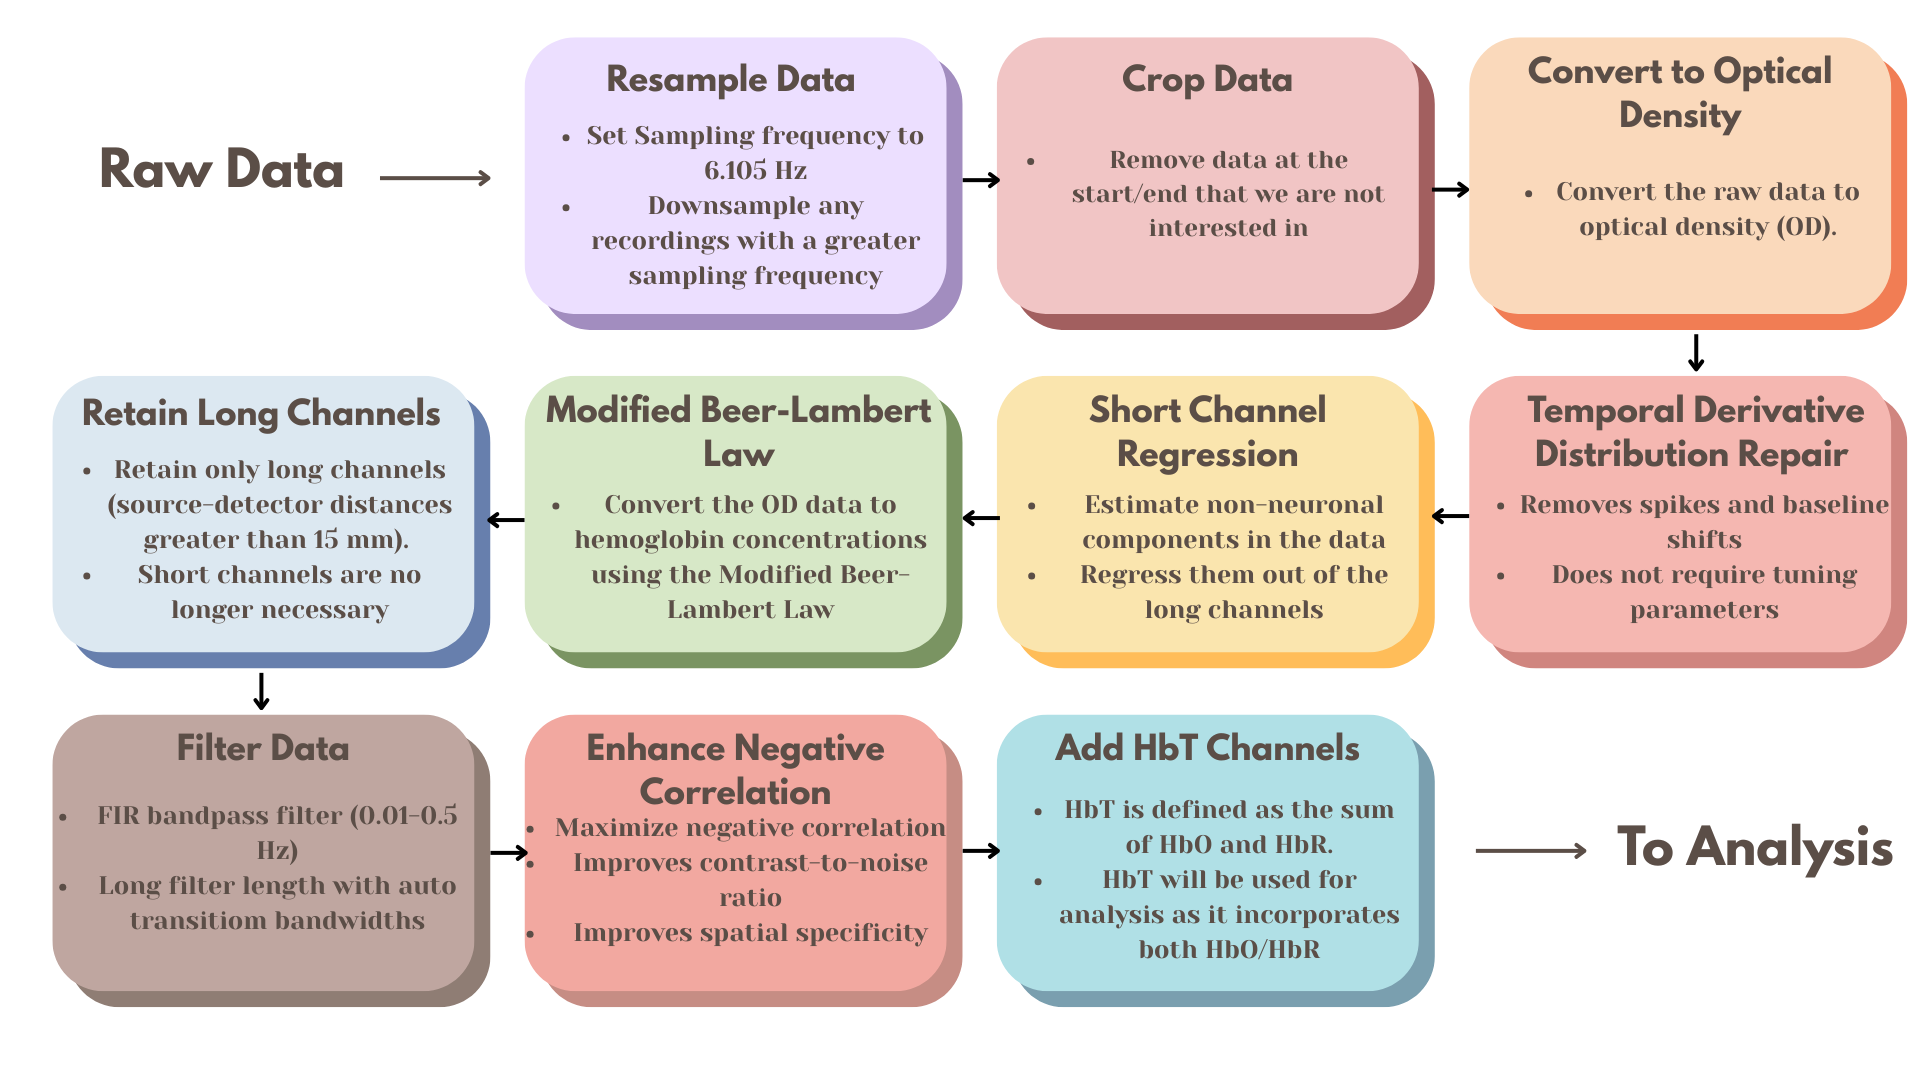
\includegraphics[width=0.95\textwidth, clip, trim=25 50 0 0]{C:/Users/super/OneDrive - Ontario Tech University/fNIRS_Emotions/plots/figures/Preprocessing Steps.png}
    \end{figure}
    \begin{itemize}
        \small
        \item Prepare raw fNIRS data for analysis by removing noise, artifacts, and irrelevant information.
        \item This ensures the data is suitable for extracting meaningful insights about brain activity.
    \end{itemize}
    \note[frame]{
        \begin{itemize}
            \item Before we can analyze the data, we have to preprocess it. 
            \item This is done through a series of steps, including converting to optical density (OD), applying motion and artifact correction algorithms, converting to hemoglobin concentrations using the modified Beer-Lambert law, and filtering the data. 
            \item This ensures that the data we are analyzing is suitable for extracting meaningful insights about brain activity.
            \item The three types of data we get from fNIRS are Oxygenated Hemoglobin, or HbO, Deoxygenated Hemoglobin, or HbR, and Total Hemoglobin, or HbT, which is the sum of HbO and HbR. 
            \item We will be using HbT for our analyses, as it utilizes the information from both HbO and HbR.
        \end{itemize}
    }
\end{frame}

\begin{frame}
    \frametitle{Analyses}
    \framesubtitle{General Linear Model (GLM)}
    \textbf{General Linear Model (GLM)}:
    \begin{itemize}
        \small
        \item Create a design matrix where each column represents one type of event/condition. 
        \item For each stimulus column, you mark onset/offset times and then “stretch” those into the shape of a typical blood-flow response. 
        \item This gives you a set of predicted response patterns—one for each condition—that you'll try to match to your actual fNIRS recordings.
        \begin{center}
            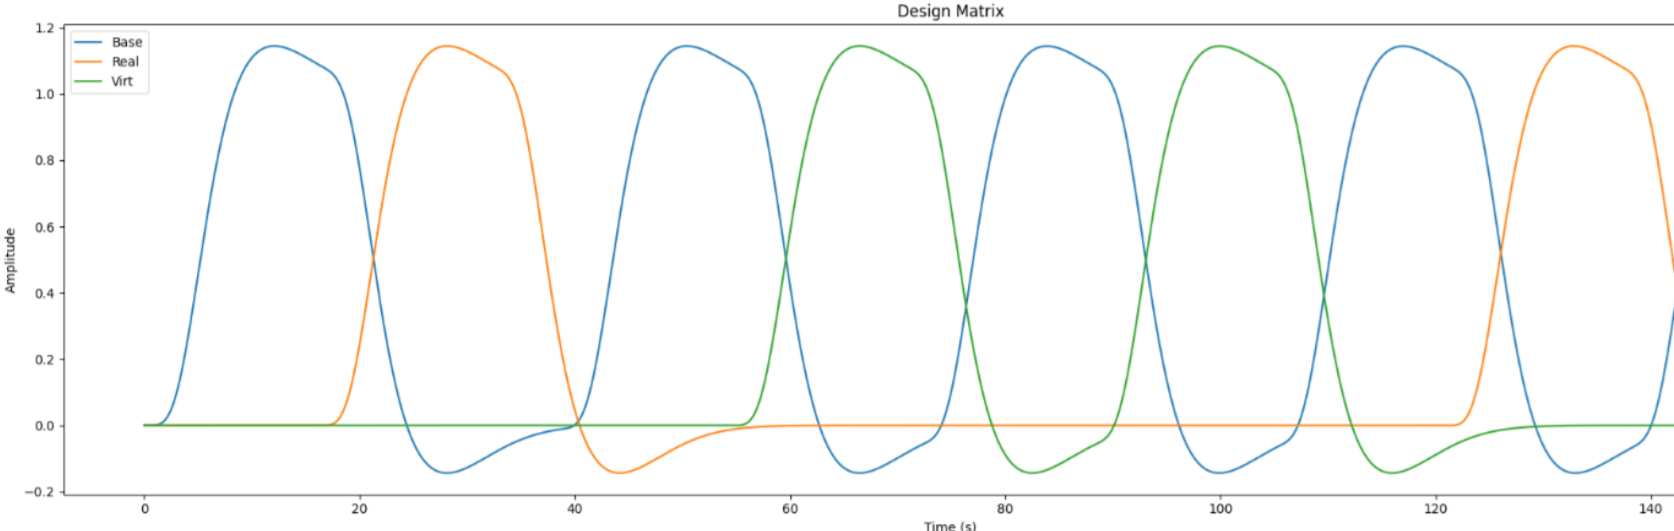
\includegraphics[width=0.9\textwidth]{C:/Users/super/OneDrive - Ontario Tech University/fNIRS_Emotions/plots/figures/Sample Design Matrix.png}
        \end{center}
        \item We then find a set of $\beta$-values (using OLS), that tell you how big the brain's blood-flow response was for each event type. 
        \item A higher $\beta$-weight means a stronger activation associated with that stimulus in that channel.
    \end{itemize}
    \note[frame]{
        \begin{itemize}
            \item So fNIRS data is extremely rich and complex, and there are many ways to analyze it, but we will be focusing on two common analyses, the first being the General Linear Model (GLM). The GLM is a tool that helps us understand how different conditions or events affect brain activity.
            \item To do this, we create a design matrix where each column represents one type of event or condition, such as real faces or virtual faces.
            \item For each stimulus column, we mark the onset/offset times of the event and then stretch those into the shape of a typical blood-flow response.
            \item This is the start/end of blocks of faces that the participants saw.
            \item This gives us a set of predicted response patterns—one for each condition—that we will try to match to our actual fNIRS recordings.
            \item We then find a set of $\beta$-values (using Ordinary Least Squares), that tell us how big the brain's blood-flow response was for each event type.
            \item Higher $\beta$-weights means stronger activation in that channel associated with that stimulus.
        \end{itemize}
    }
\end{frame}

\begin{frame}
    \frametitle{Analyses}
    \framesubtitle{Functional Connectivity (FC)}
    \begin{columns}
        \begin{column}{0.5\textwidth}
            \begin{itemize}
                \small
                \item \textbf{Functional connectivity (FC)} describes how blood-flow signals from different brain regions fluctuate together over time, showing which areas of the brain are working in sync.
                \item We apply a continuous wavelet transform (CWT) using a Morlet wavelet focused on the 0.2-0.5 Hz band.
                \item The CWT gives us coherence scores (ranging from 0 to 1) for frequencies within that band. 
            \end{itemize}
        \end{column}
        \begin{column}{0.5\textwidth}
            \begin{figure}
                \centering
                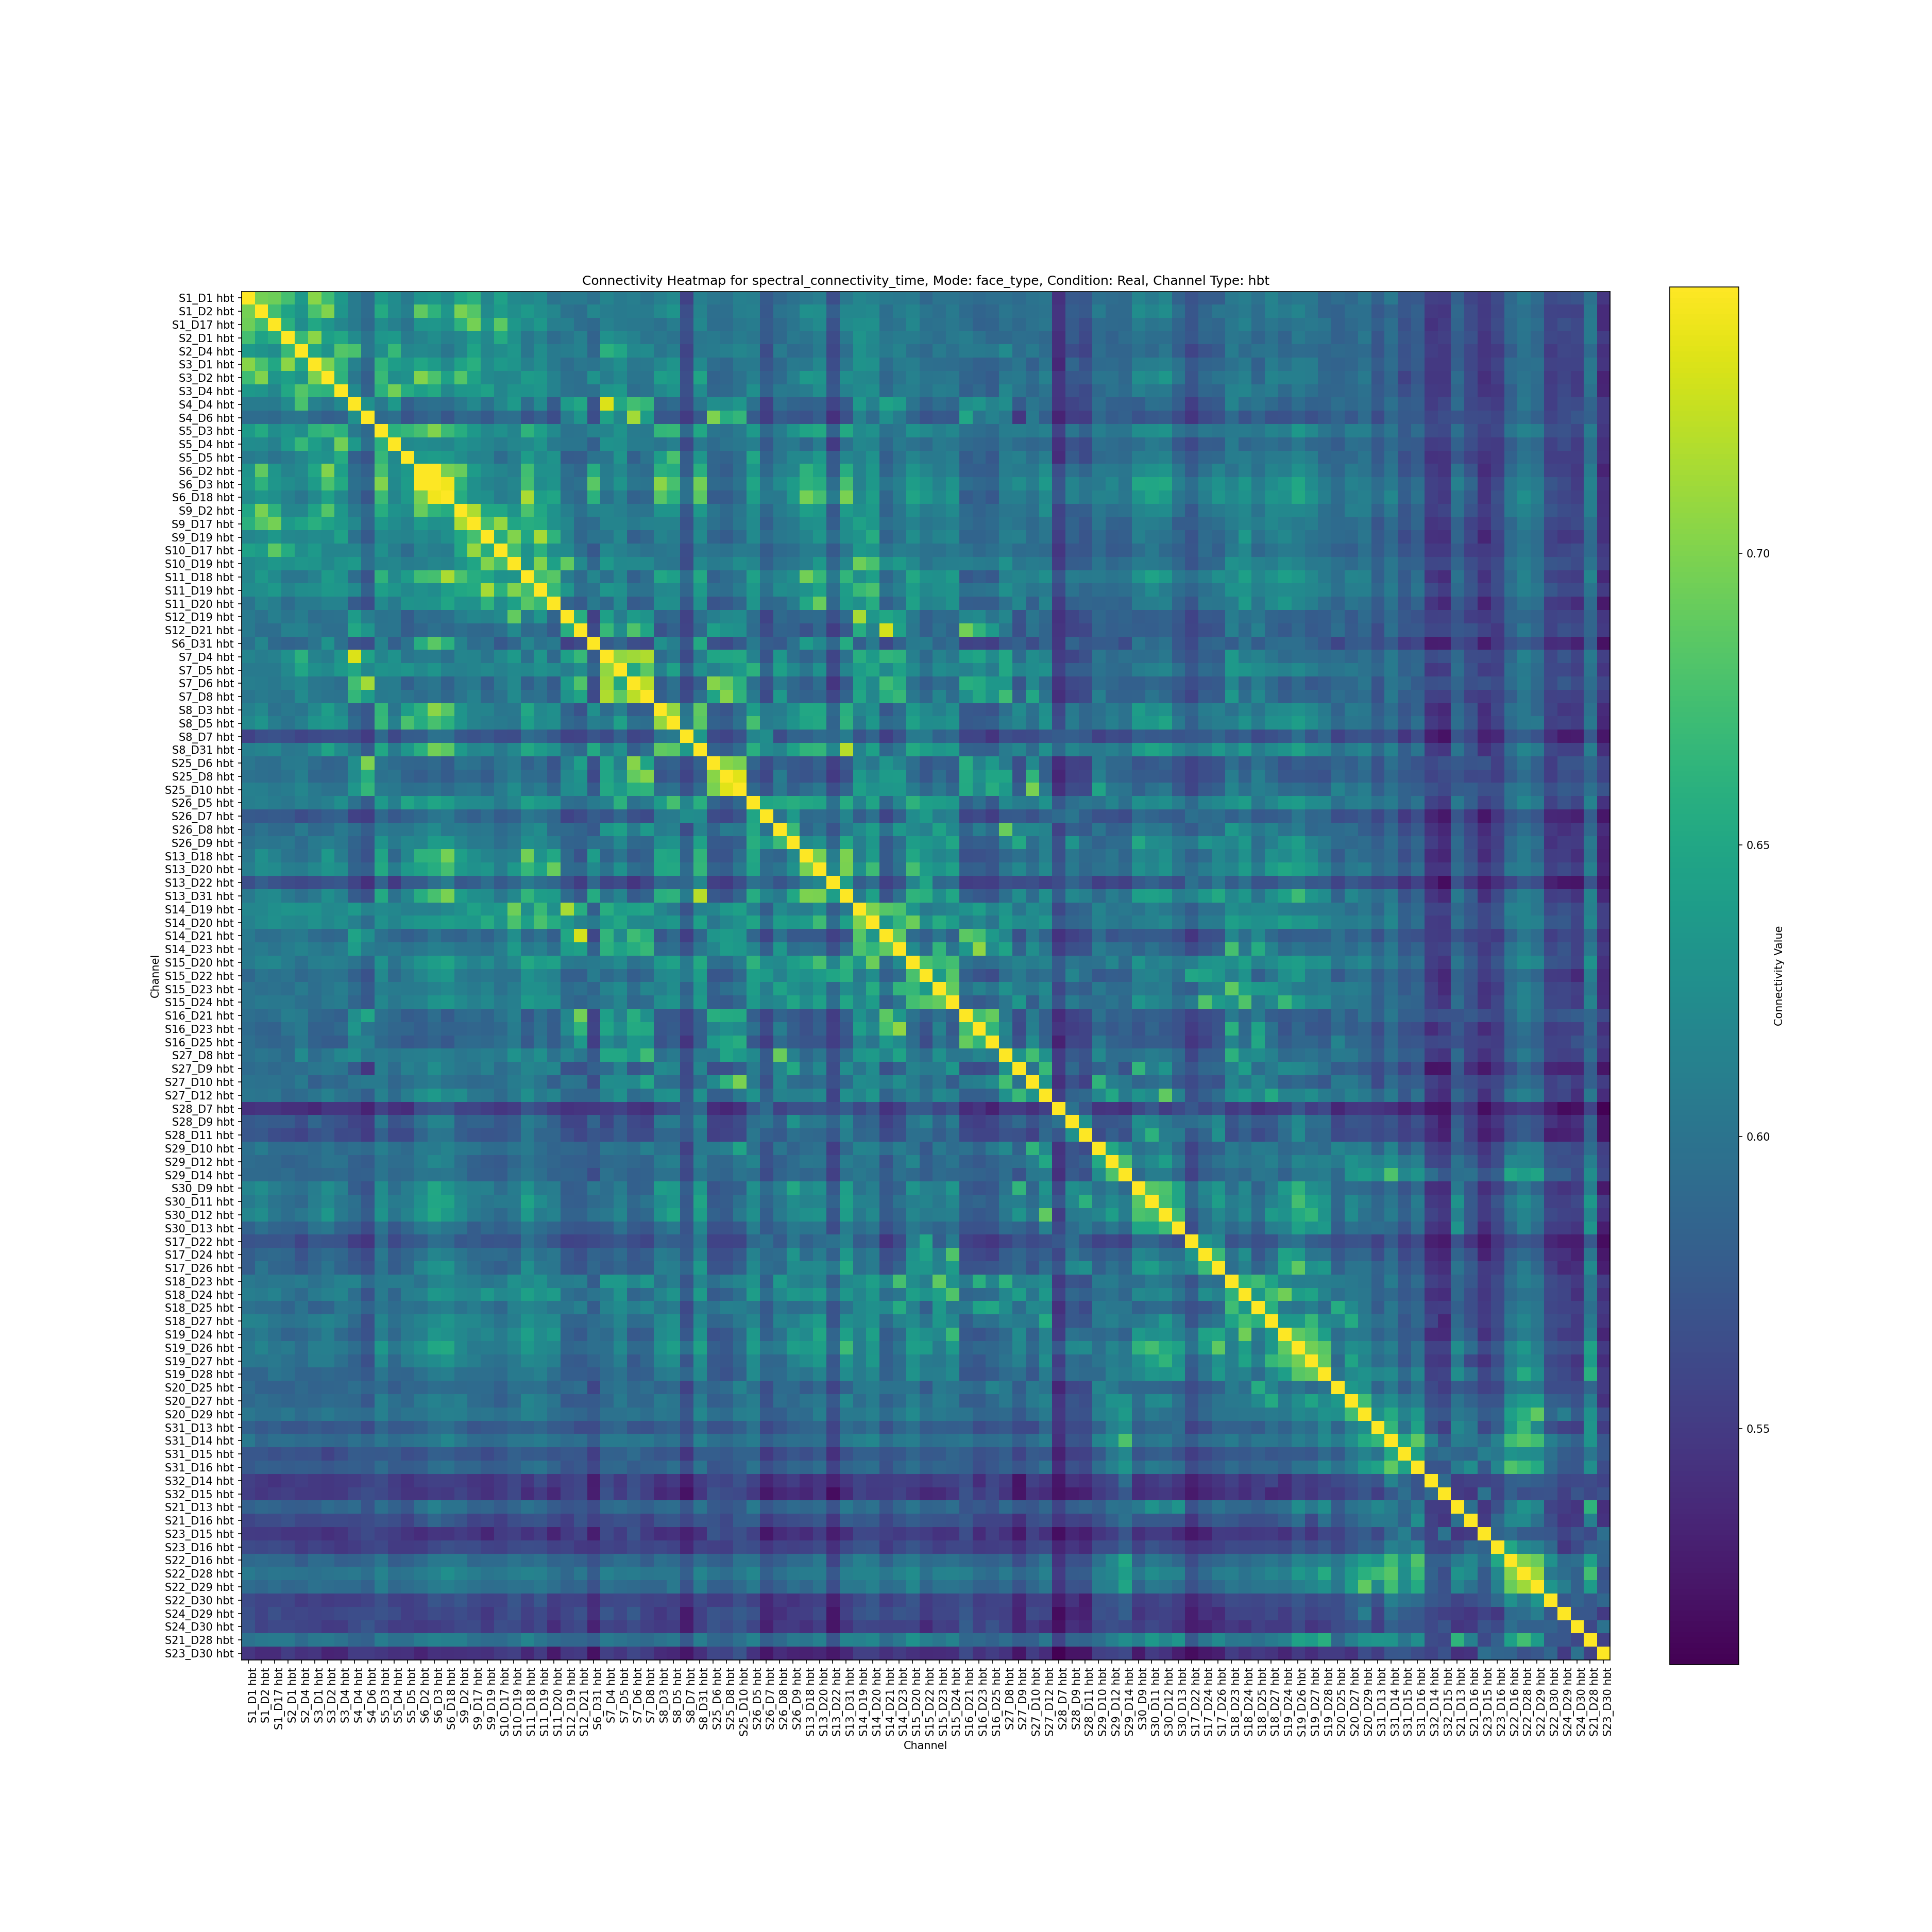
\includegraphics[width=1\textwidth]{C:/Users/super/OneDrive - Ontario Tech University/fNIRS_Emotions/plots/spectral_connectivity_time/chord_plots/conditions/face_type_Real_con.png}
            \end{figure}
        \end{column}
    \end{columns}
    \begin{itemize}
        \small
        \item In summary, by looking at how similar these averaged coherence values are between every pair of regions over time, we can see which brain areas synchronize their activity under different conditions.
    \end{itemize}
    \note[frame]{
        \begin{itemize}
            \item The second analysis we will be looking at is functional connectivity (FC). 
            \item FC is like figuring out which parts of the brain are "in sync" or working together by looking at how their activity changes over time.
            \item To do this, we use a tool called continuous wavelet transform (CWT), which helps us zoom in on specific brain activity patterns in a certain range (0.2-0.5 Hz). 
            \item The CWT gives us scores between 0 and 1, where 1 means two brain areas are perfectly synchronized, and 0 means they are not at all synchronized.
            \item By averaging these scores across participants, we can see which brain areas are most connected and how this changes depending on the condition (e.g., real vs. virtual faces).
            \item This is an example of the FC for the real face condition, each of the 103 channels is connected to every other channel, and the brighter the line, the more synchronized the neural activity is between those two channels.
        \end{itemize}
    }
\end{frame}

\begin{frame}
    \frametitle{Results}
    \framesubtitle{Real vs. Virtual Faces}
    \begin{figure}
        \centering
        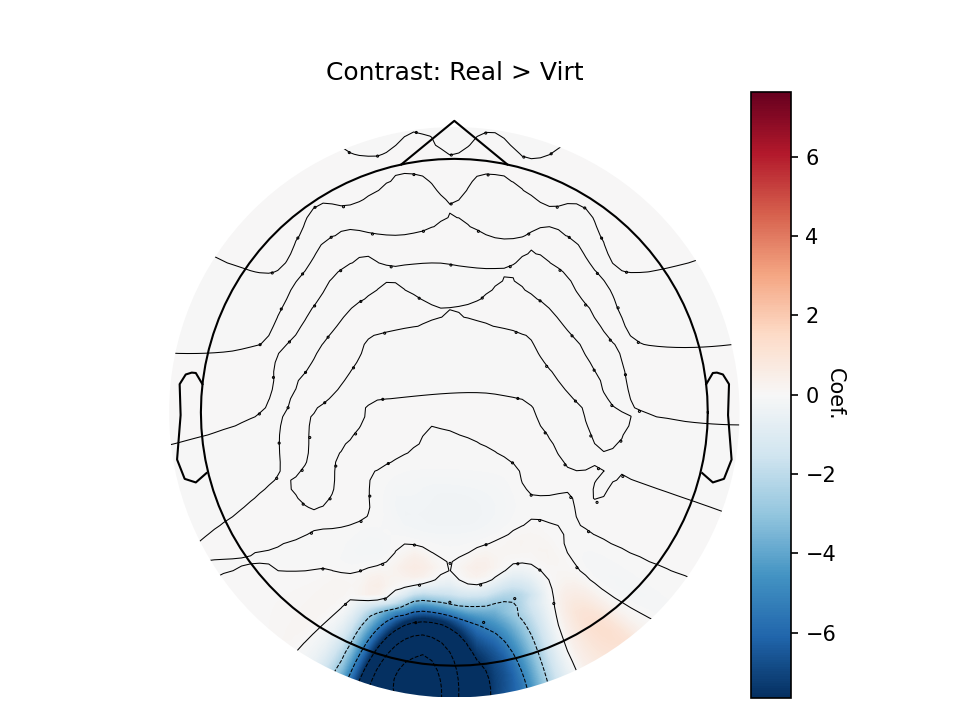
\includegraphics[width=0.7\textwidth, clip, trim=40 0 160 0]{C:/Users/super/OneDrive - Ontario Tech University/fNIRS_Emotions/plots/glm/contrasts/differences/Contrast_Real-Virt.png}
    \end{figure}
    \begin{itemize}
        \small
        \item GLM contrast for Real vs. Virtual Faces.  
        \item Left Occipital region has slightly more activation for Virtual Faces. 
    \end{itemize}
    \note[frame]{
        \begin{itemize}
            \item So finally, it's time to look at the results of our analyses for real vs. virtual faces.
            \item Here we have the GLM contrast for real vs. virtual faces, which shows the differences in activation between the two conditions.
            \item The way to read the GLM contrast is that if the color is red, it means that the real faces have more activation than virtual faces, and if the color is blue, it means that virtual faces have more activation than real faces.
            \item We see the left occipital region has one channel that has higher activation for virtual faces compared to real faces. 
        \end{itemize}
    }
\end{frame}

\begin{frame}
    \frametitle{Results}
    \framesubtitle{Real vs. Virtual Faces}
    \begin{figure}
        \centering
        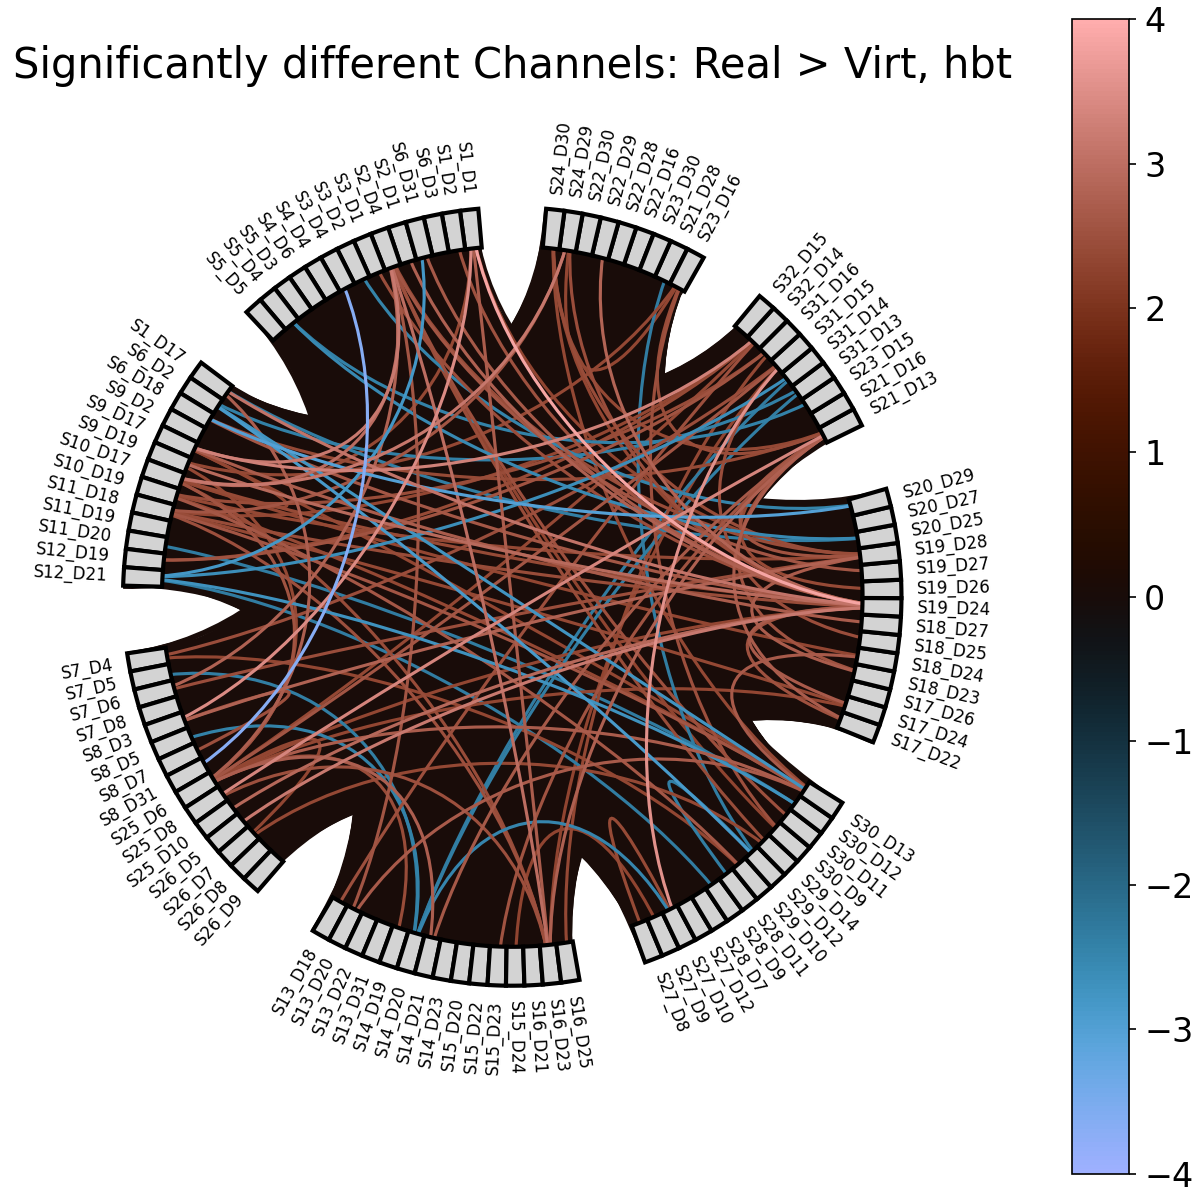
\includegraphics[width=0.525\textwidth]{C:/Users/super/OneDrive - Ontario Tech University/fNIRS_Emotions/plots/spectral_connectivity_time/chord_plots/group_level_t_tests_roi/face_type_Real_Virt.png}
    \end{figure}
    \begin{itemize}
        \small
        \item Significant differences in connectivity between regions for Real vs. Virtual Faces.
        \item We see most differences in connectivity between Left Frontal-Left Parietal and Left Prefrontal-Right Occipital regions.
    \end{itemize}
    \note[frame]{
        \begin{itemize}
            \item Here we have the difference in connectivity between regions for real and virtual faces, we interpret this by looking at the brightness of the lines again where the darker the line, the less synchronized the neural activity is between those two regions.
            \item We see the most significant differences in connectivity between the left frontal and left parietal regions, and between the left prefrontal and right occipital regions.
        \end{itemize}
    }
\end{frame}

\begin{frame}
    \frametitle{Results}
    \framesubtitle{Emotional Faces}
    \begin{center}
        \textbf{Neutral vs. All Other Emotions}
    \end{center}
    \begin{figure}
        \begin{figure}
            \centering
            \begin{tabular}{ccc}
                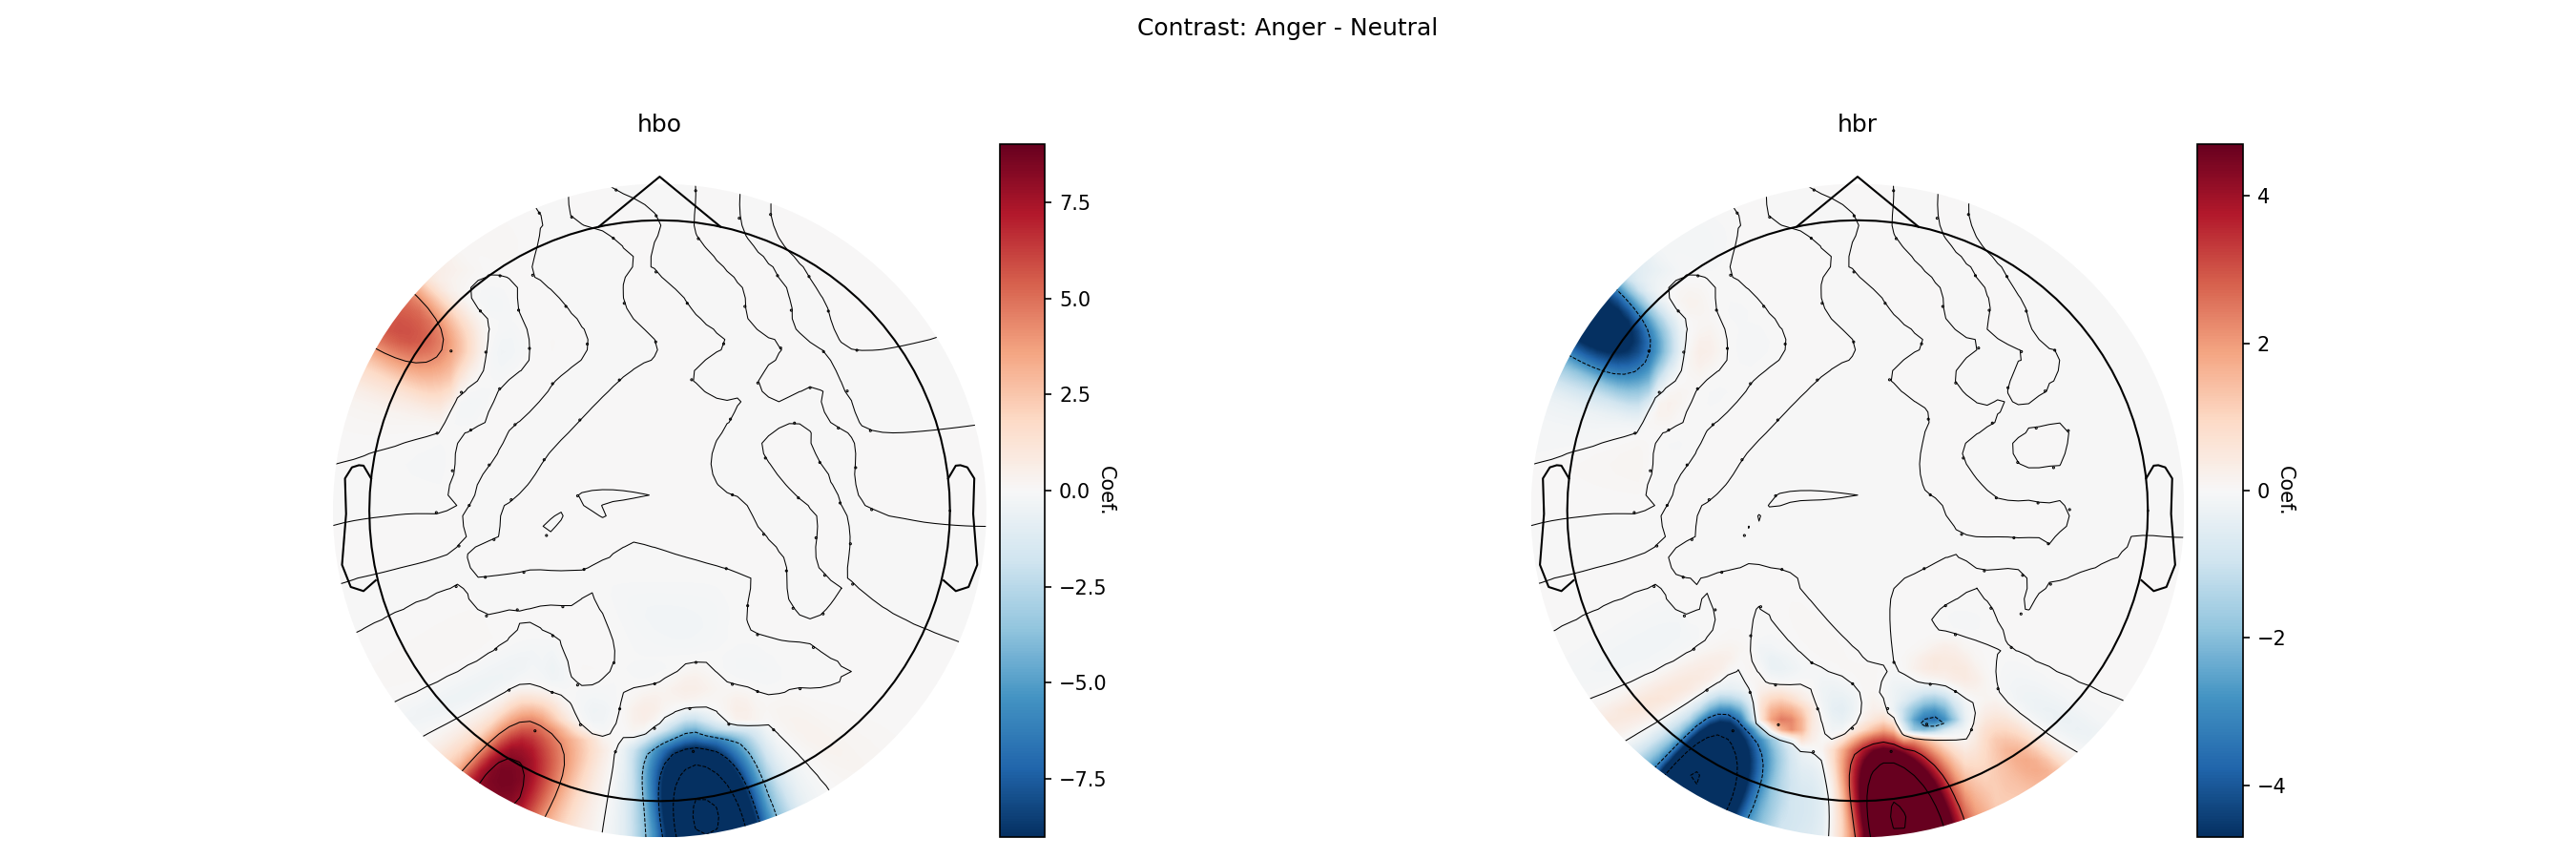
\includegraphics[width=0.29\textwidth, clip, trim=40 0 160 0]{C:/Users/super/OneDrive - Ontario Tech University/fNIRS_Emotions/plots/glm/contrasts/differences_neutral/Contrast_Anger-Neutral.png} &
                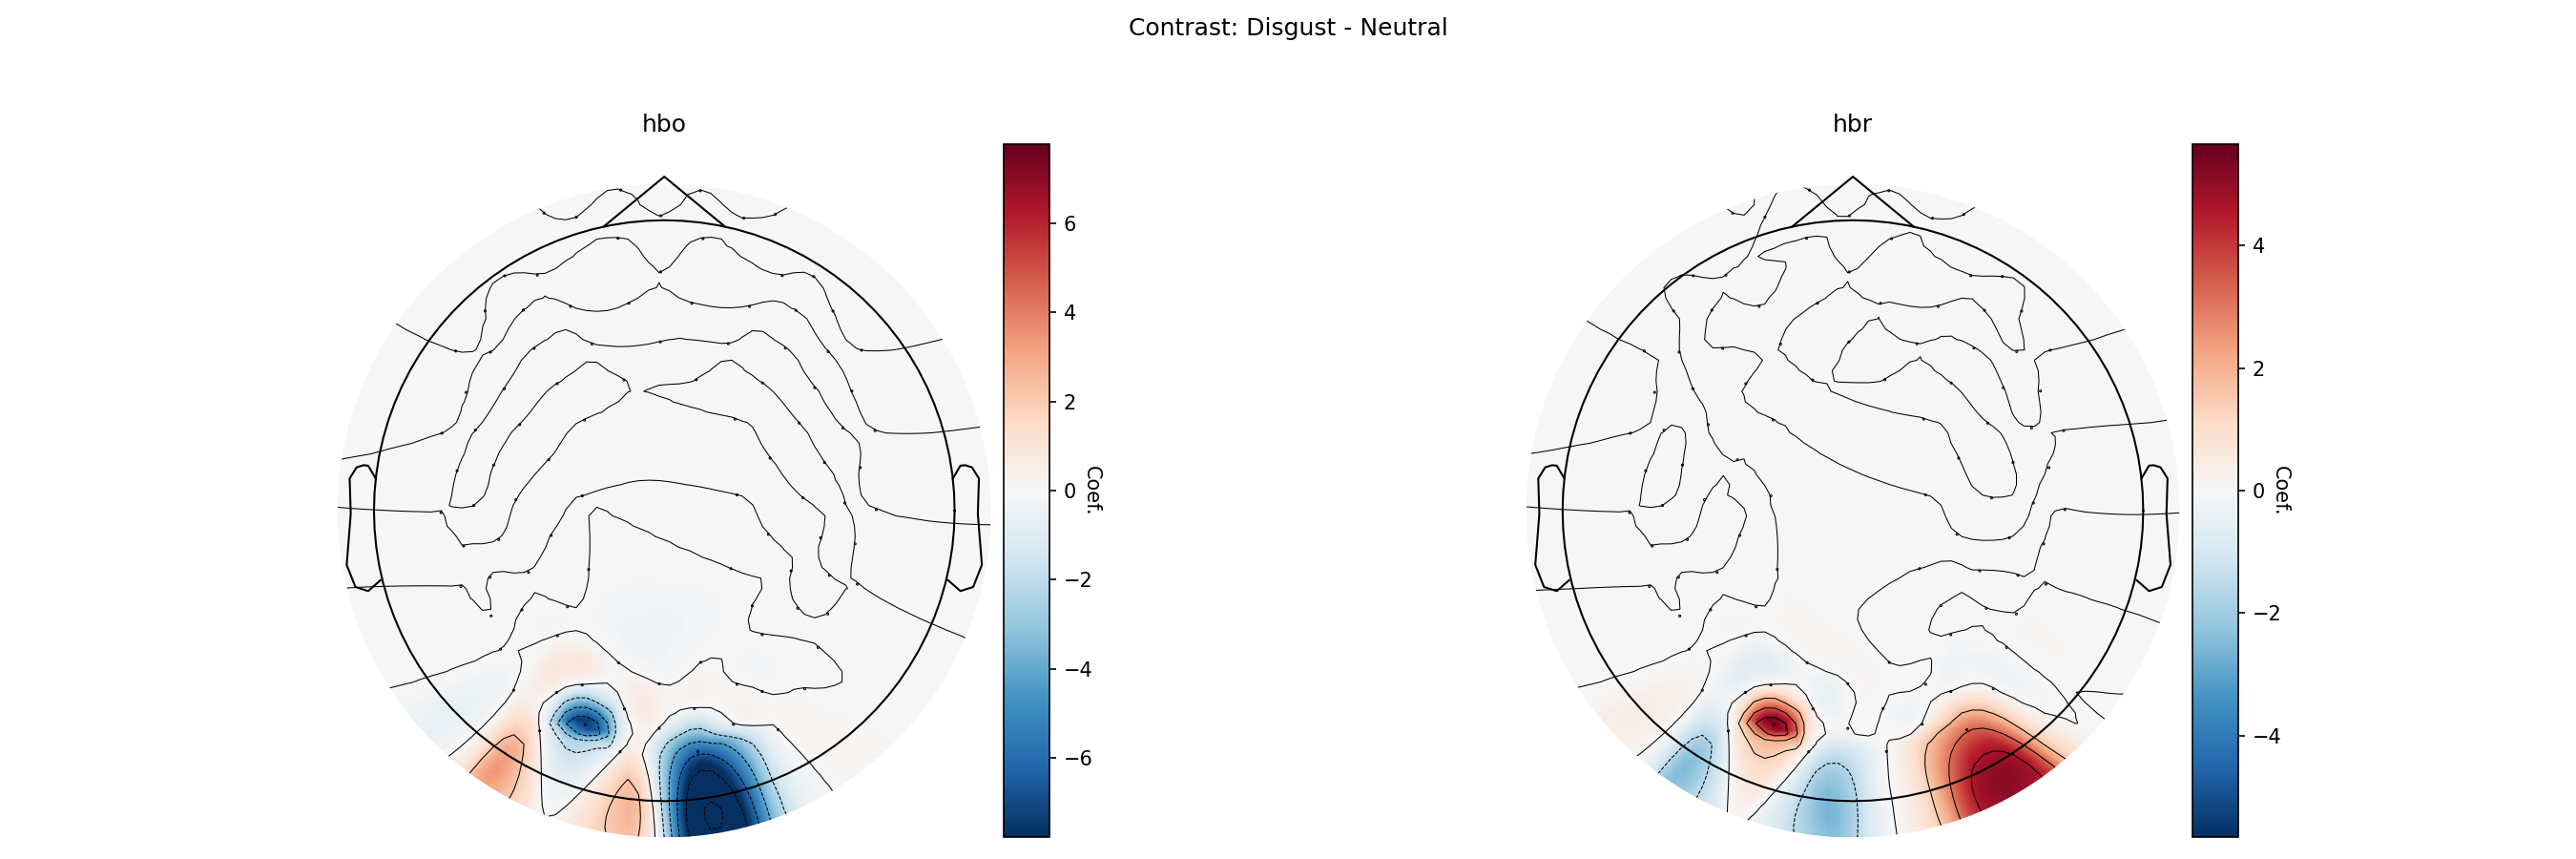
\includegraphics[width=0.29\textwidth, clip, trim=40 0 160 0]{C:/Users/super/OneDrive - Ontario Tech University/fNIRS_Emotions/plots/glm/contrasts/differences_neutral/Contrast_Disgust-Neutral.png} &
                
\includegraphics[width=0.29\textwidth, clip, trim=40 0 160 0]{C:/Users/super/OneDrive - Ontario Tech University/fNIRS_Emotions/plots/glm/contrasts/differences_neutral/Contrast_Fear-Neutral.png} \\
                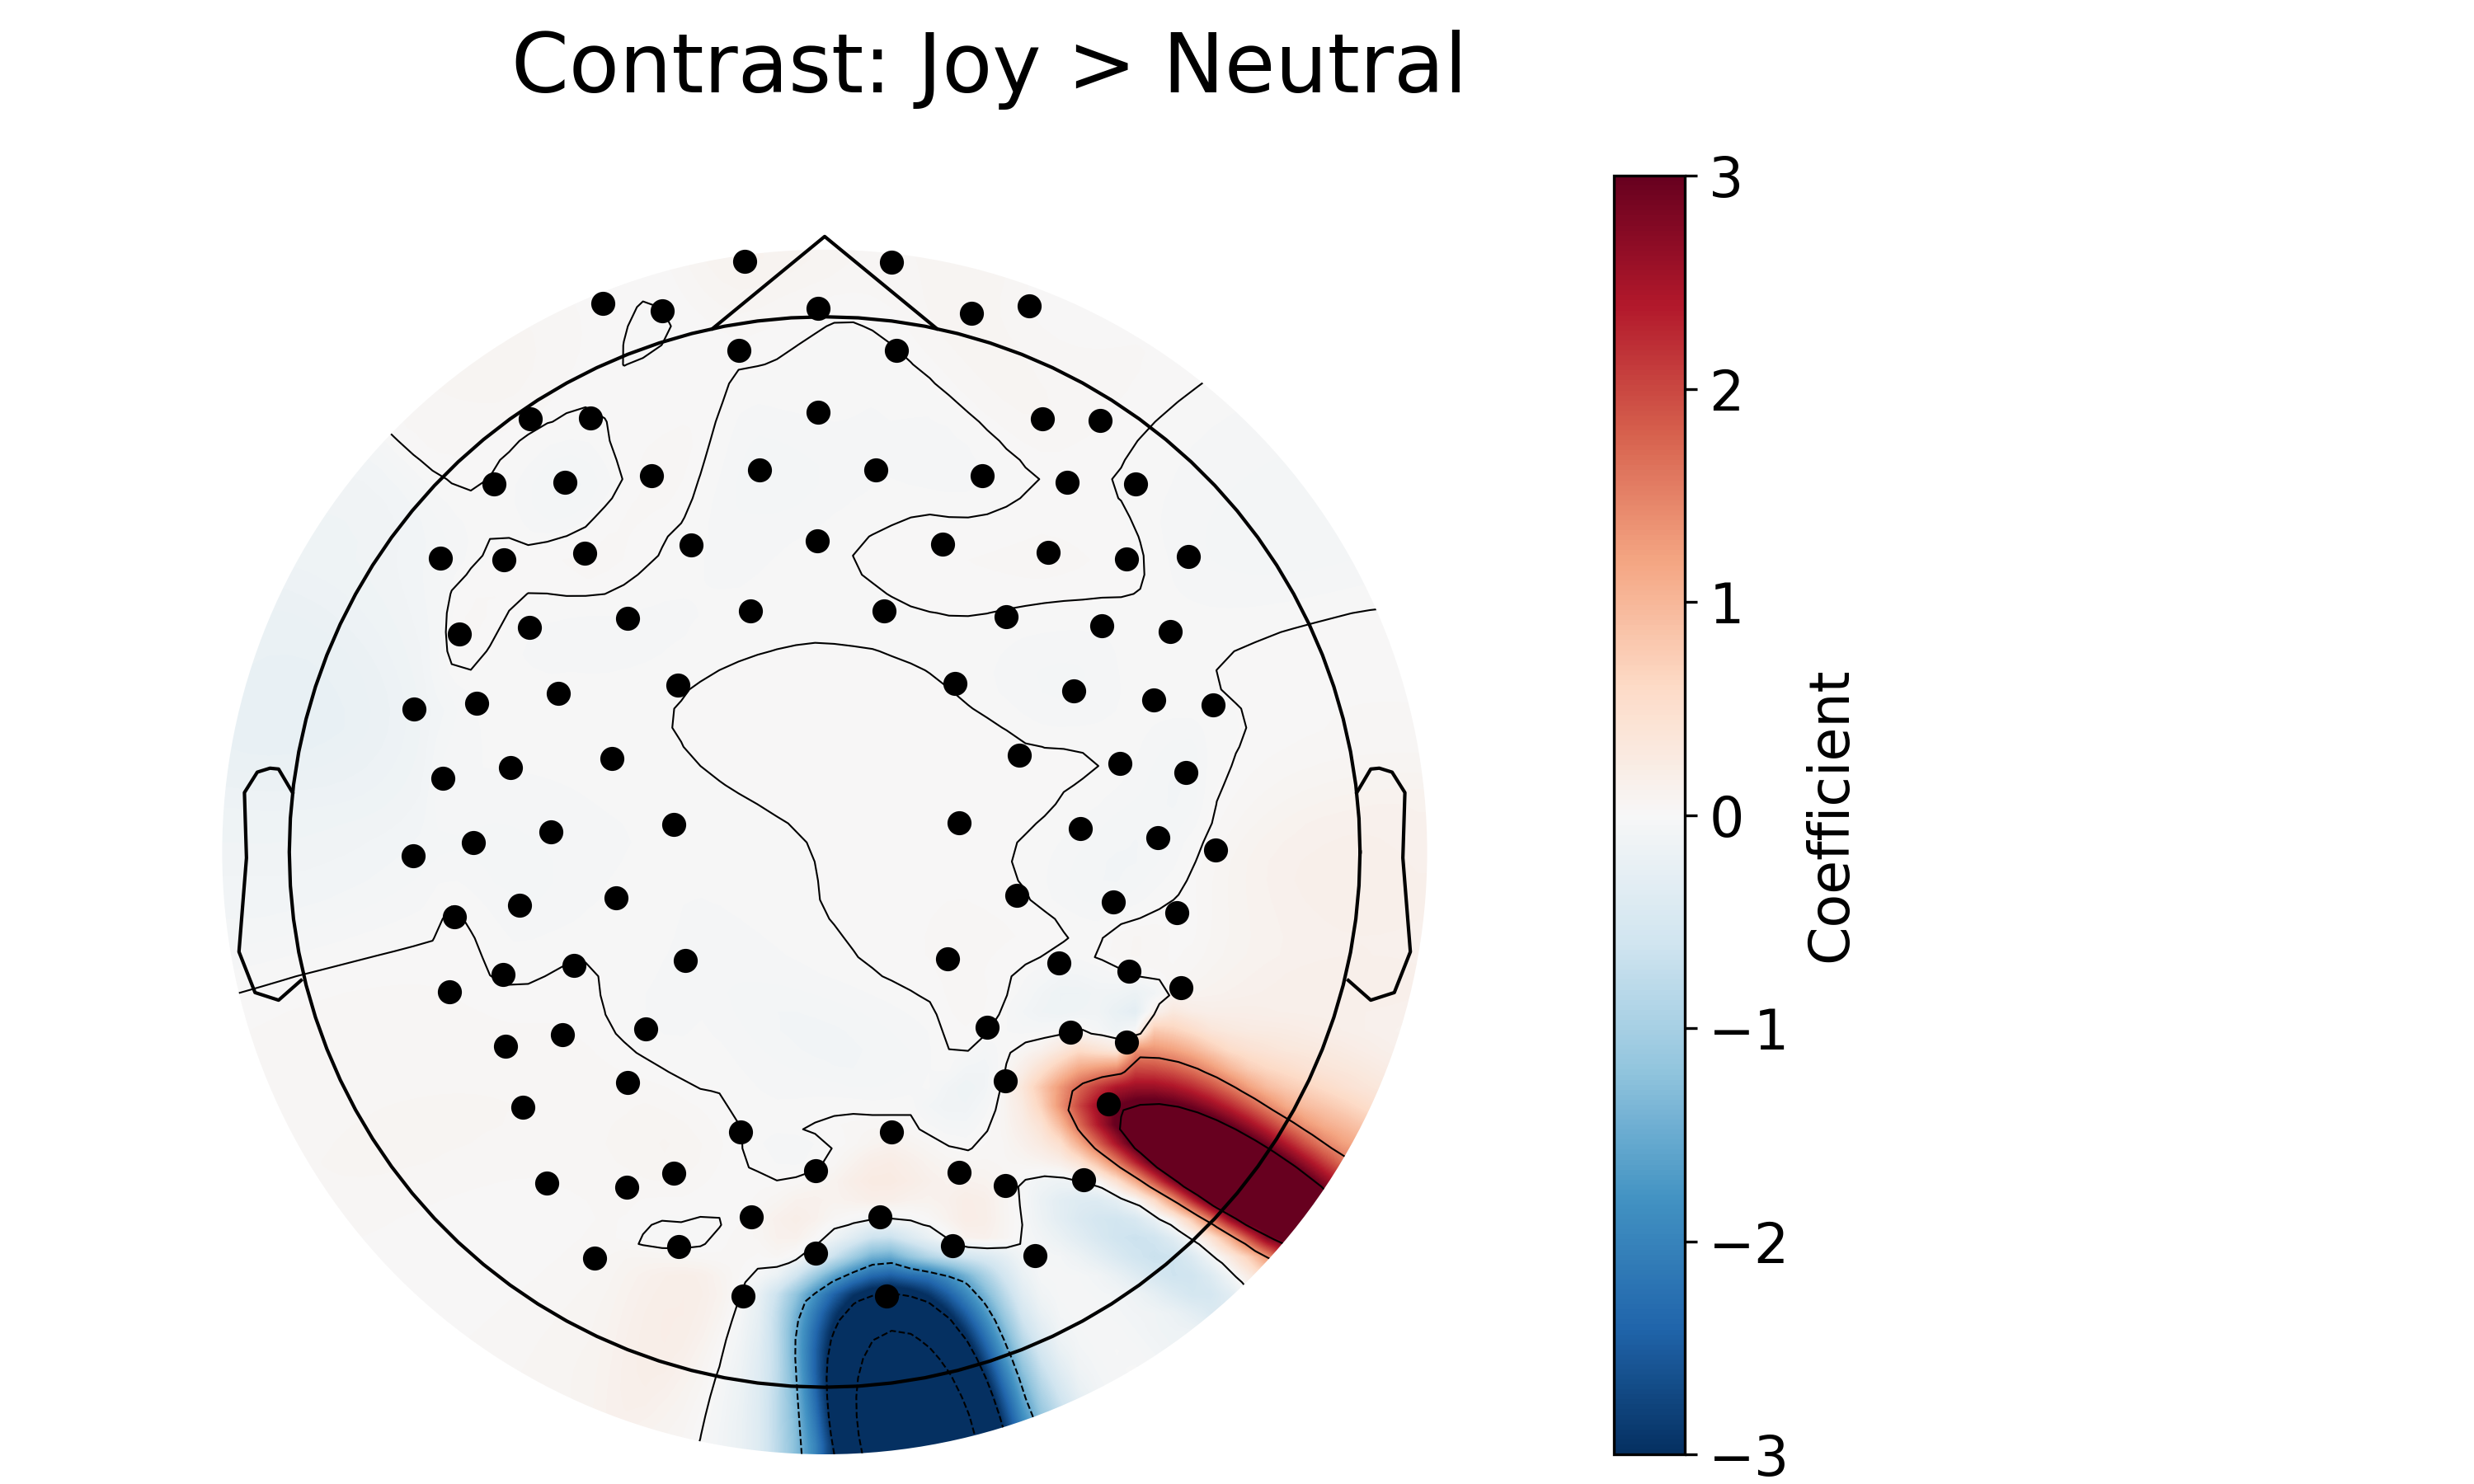
\includegraphics[width=0.29\textwidth, clip, trim=40 0 160 0]{C:/Users/super/OneDrive - Ontario Tech University/fNIRS_Emotions/plots/glm/contrasts/differences_neutral/Contrast_Joy-Neutral.png} &
                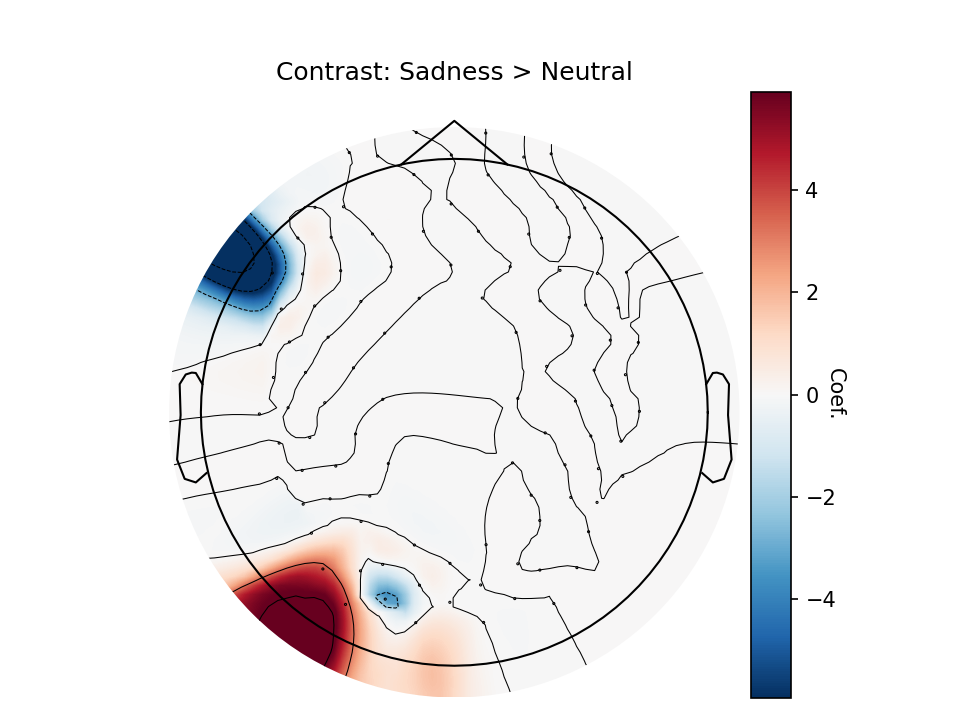
\includegraphics[width=0.29\textwidth, clip, trim=40 0 160 0]{C:/Users/super/OneDrive - Ontario Tech University/fNIRS_Emotions/plots/glm/contrasts/differences_neutral/Contrast_Sadness-Neutral.png} &
                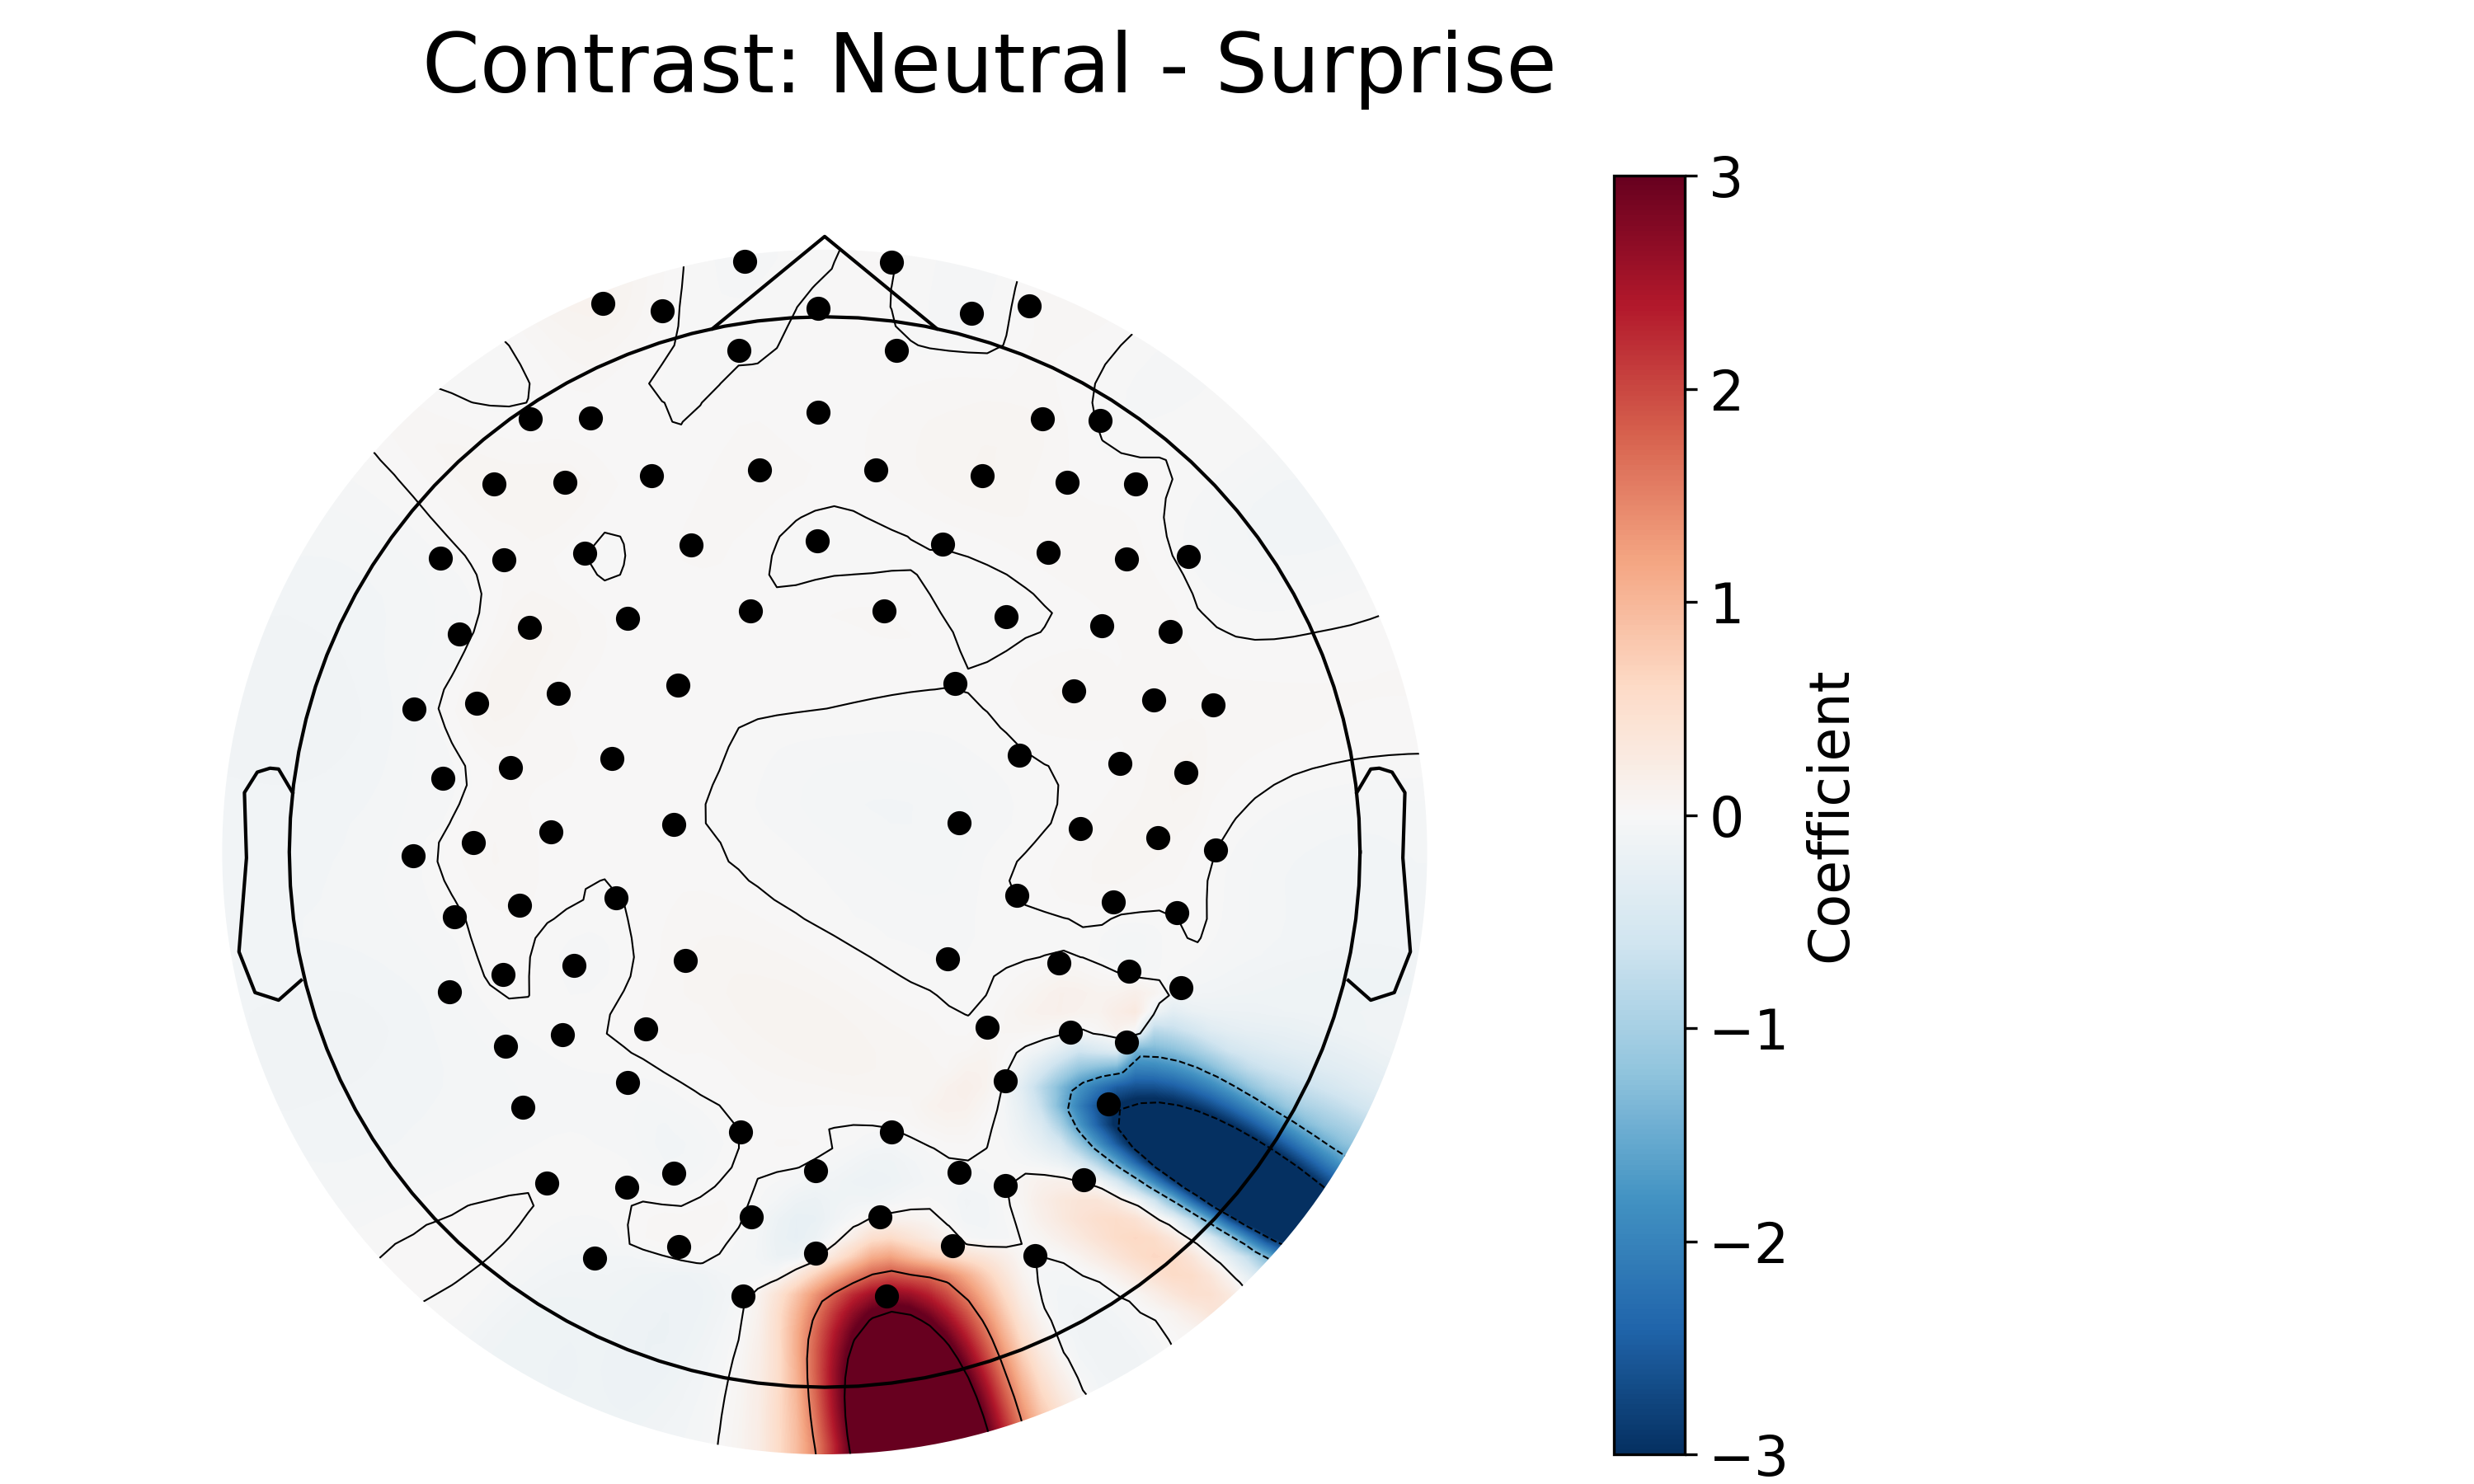
\includegraphics[width=0.29\textwidth, clip, trim=40 0 160 0]{C:/Users/super/OneDrive - Ontario Tech University/fNIRS_Emotions/plots/glm/contrasts/differences_neutral/Contrast_Neutral-Surprise.png} \\
            \end{tabular}
        \end{figure}
    \end{figure}
    \begin{itemize}
        \small
        \item The GLM contrast for Neutral vs. all other emotions shows differences in activation in multiple regions. (except disgust)
    \end{itemize}
    \note[frame]{
        \begin{itemize}
            \item Now, on to the results for the emotional faces.
            \item The emotion Neutral shows significant differences in activation from all of the other emotions in multiple regions, except for disgust.
            \item The way to read this is the same as before, if the color is red, it means that the other emotion has more activation than neutral, and if the color is blue, it means that neutral has more activation than the other emotion.
        \end{itemize}
    }
\end{frame}

\begin{frame}
    \frametitle{Results}
    \framesubtitle{Emotional Faces}
    \begin{center}
        \textbf{Surprise vs. All Other Emotions}
    \end{center}
    \begin{figure}
        \begin{figure}
            \centering
            \begin{tabular}{ccc}
                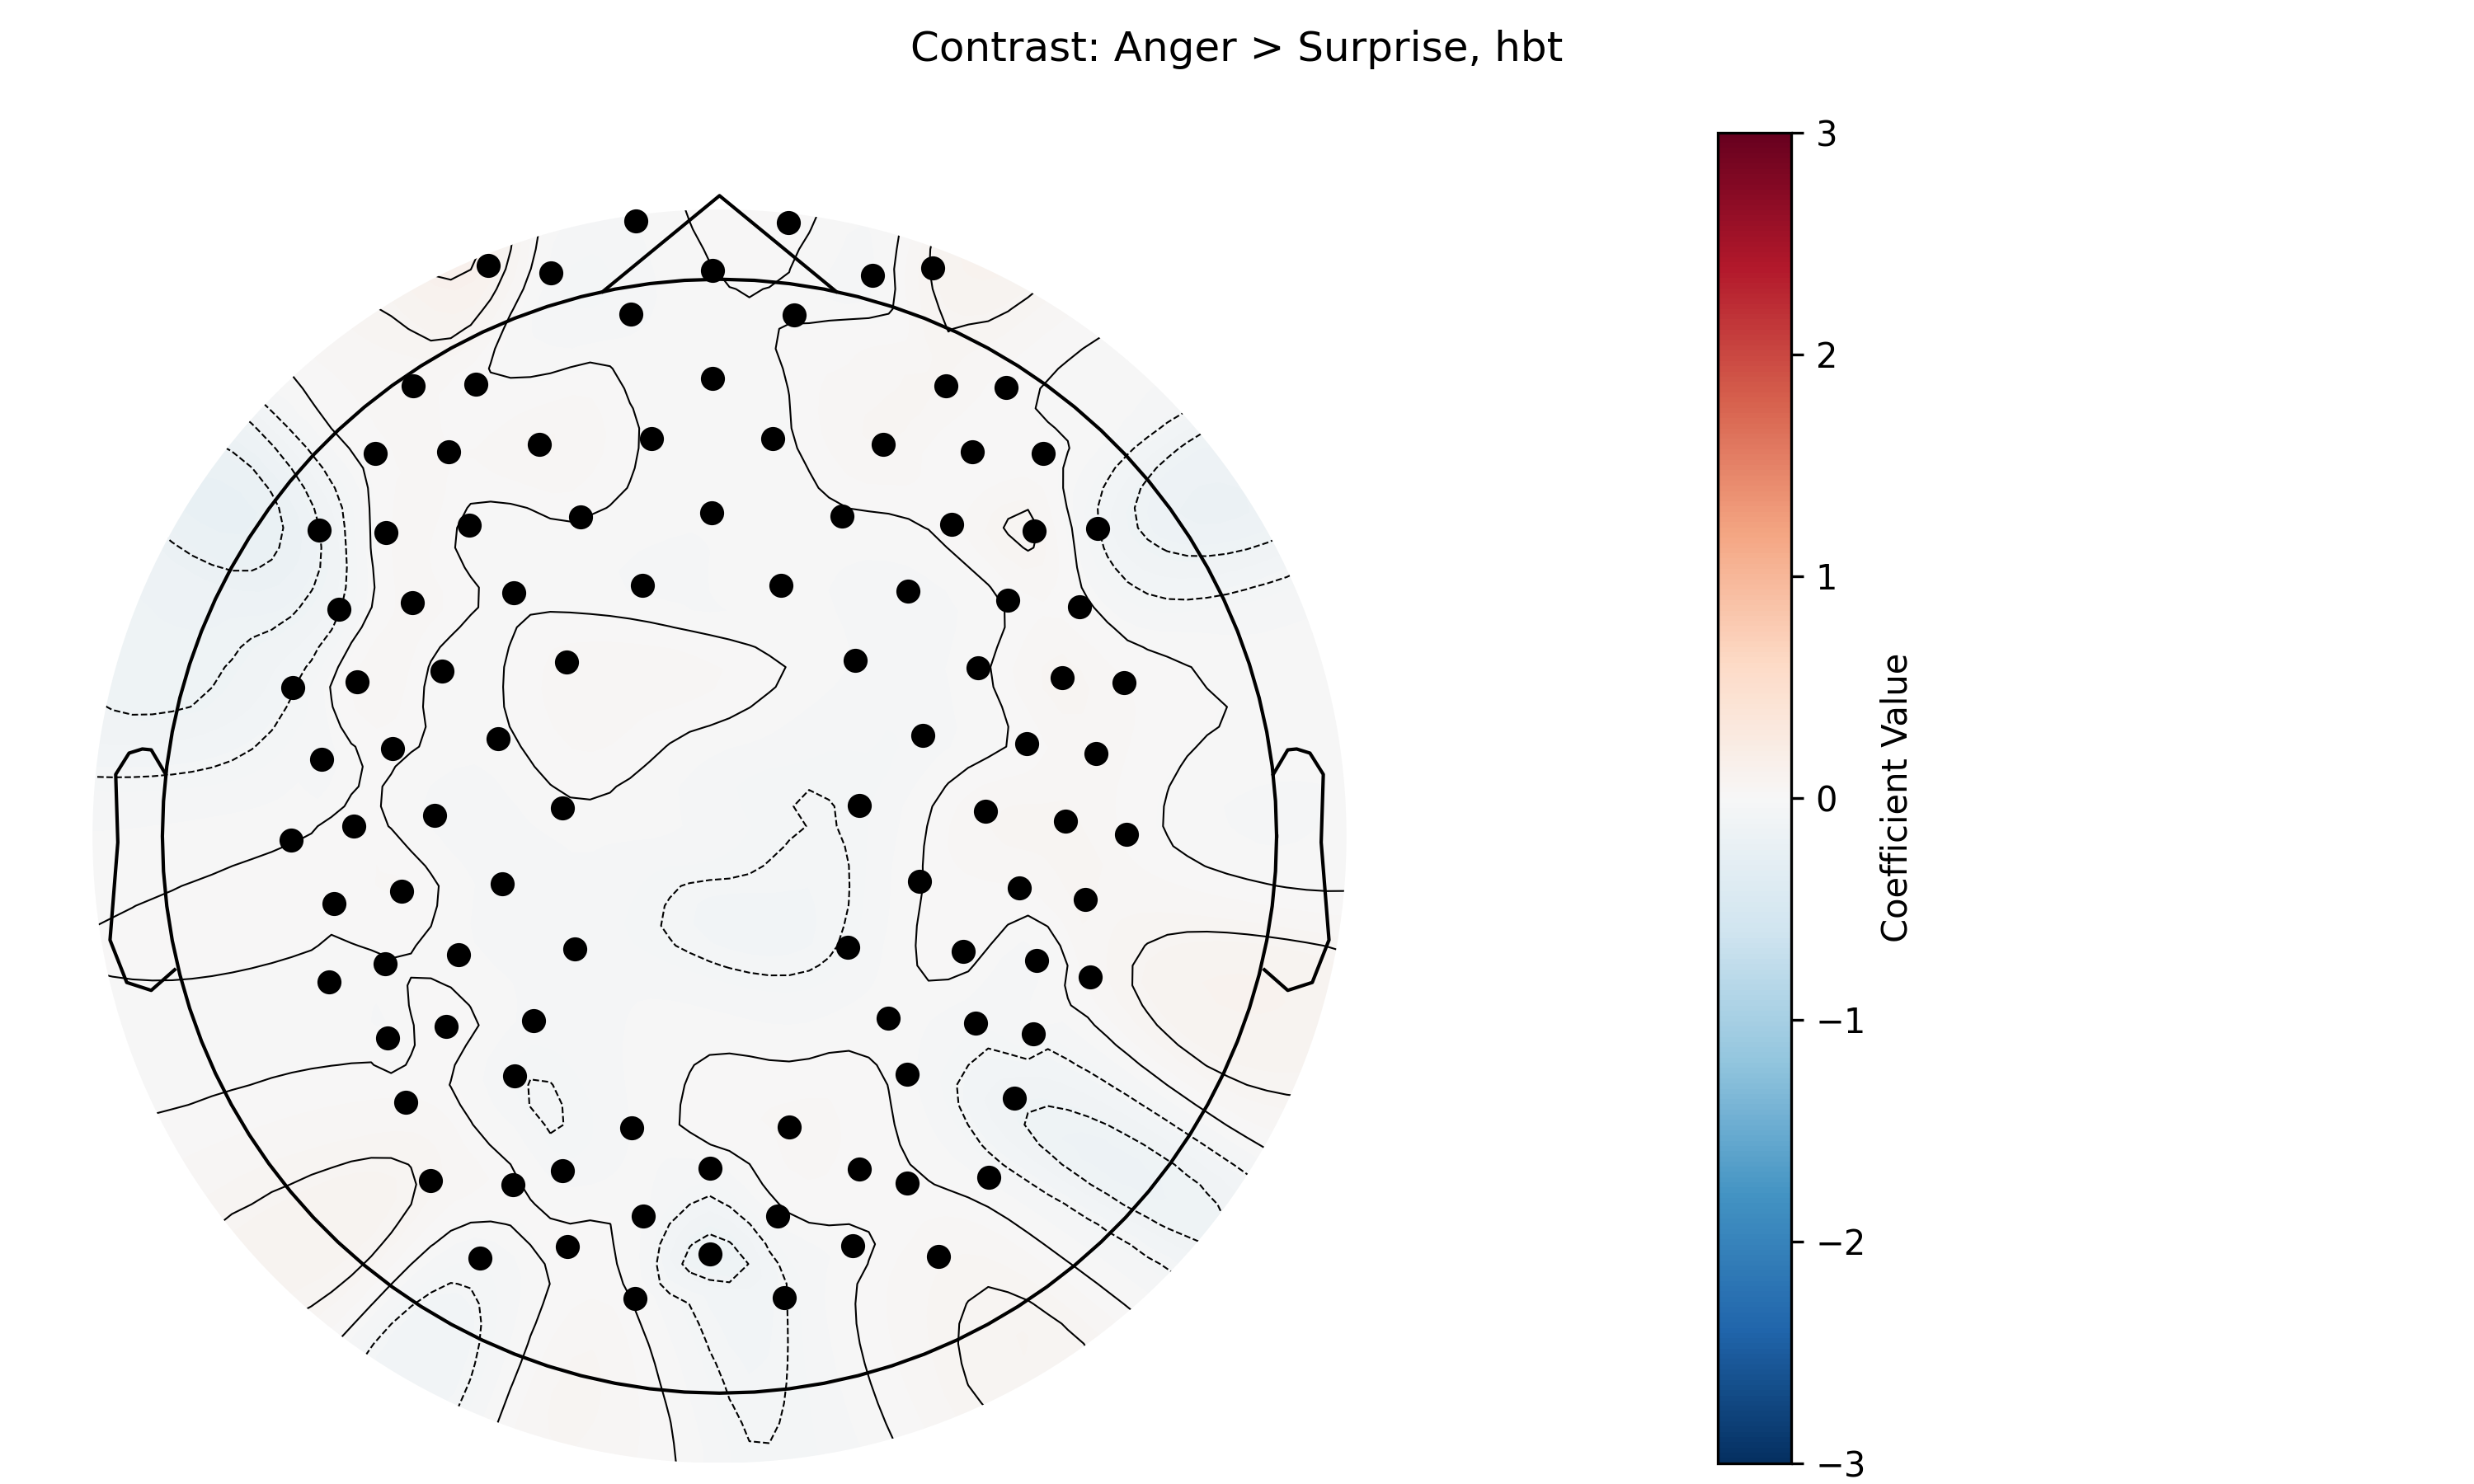
\includegraphics[width=0.29\textwidth, clip, trim=40 0 160 0]{C:/Users/super/OneDrive - Ontario Tech University/fNIRS_Emotions/plots/glm/contrasts/differences/Contrast_Anger-Surprise.png} &
                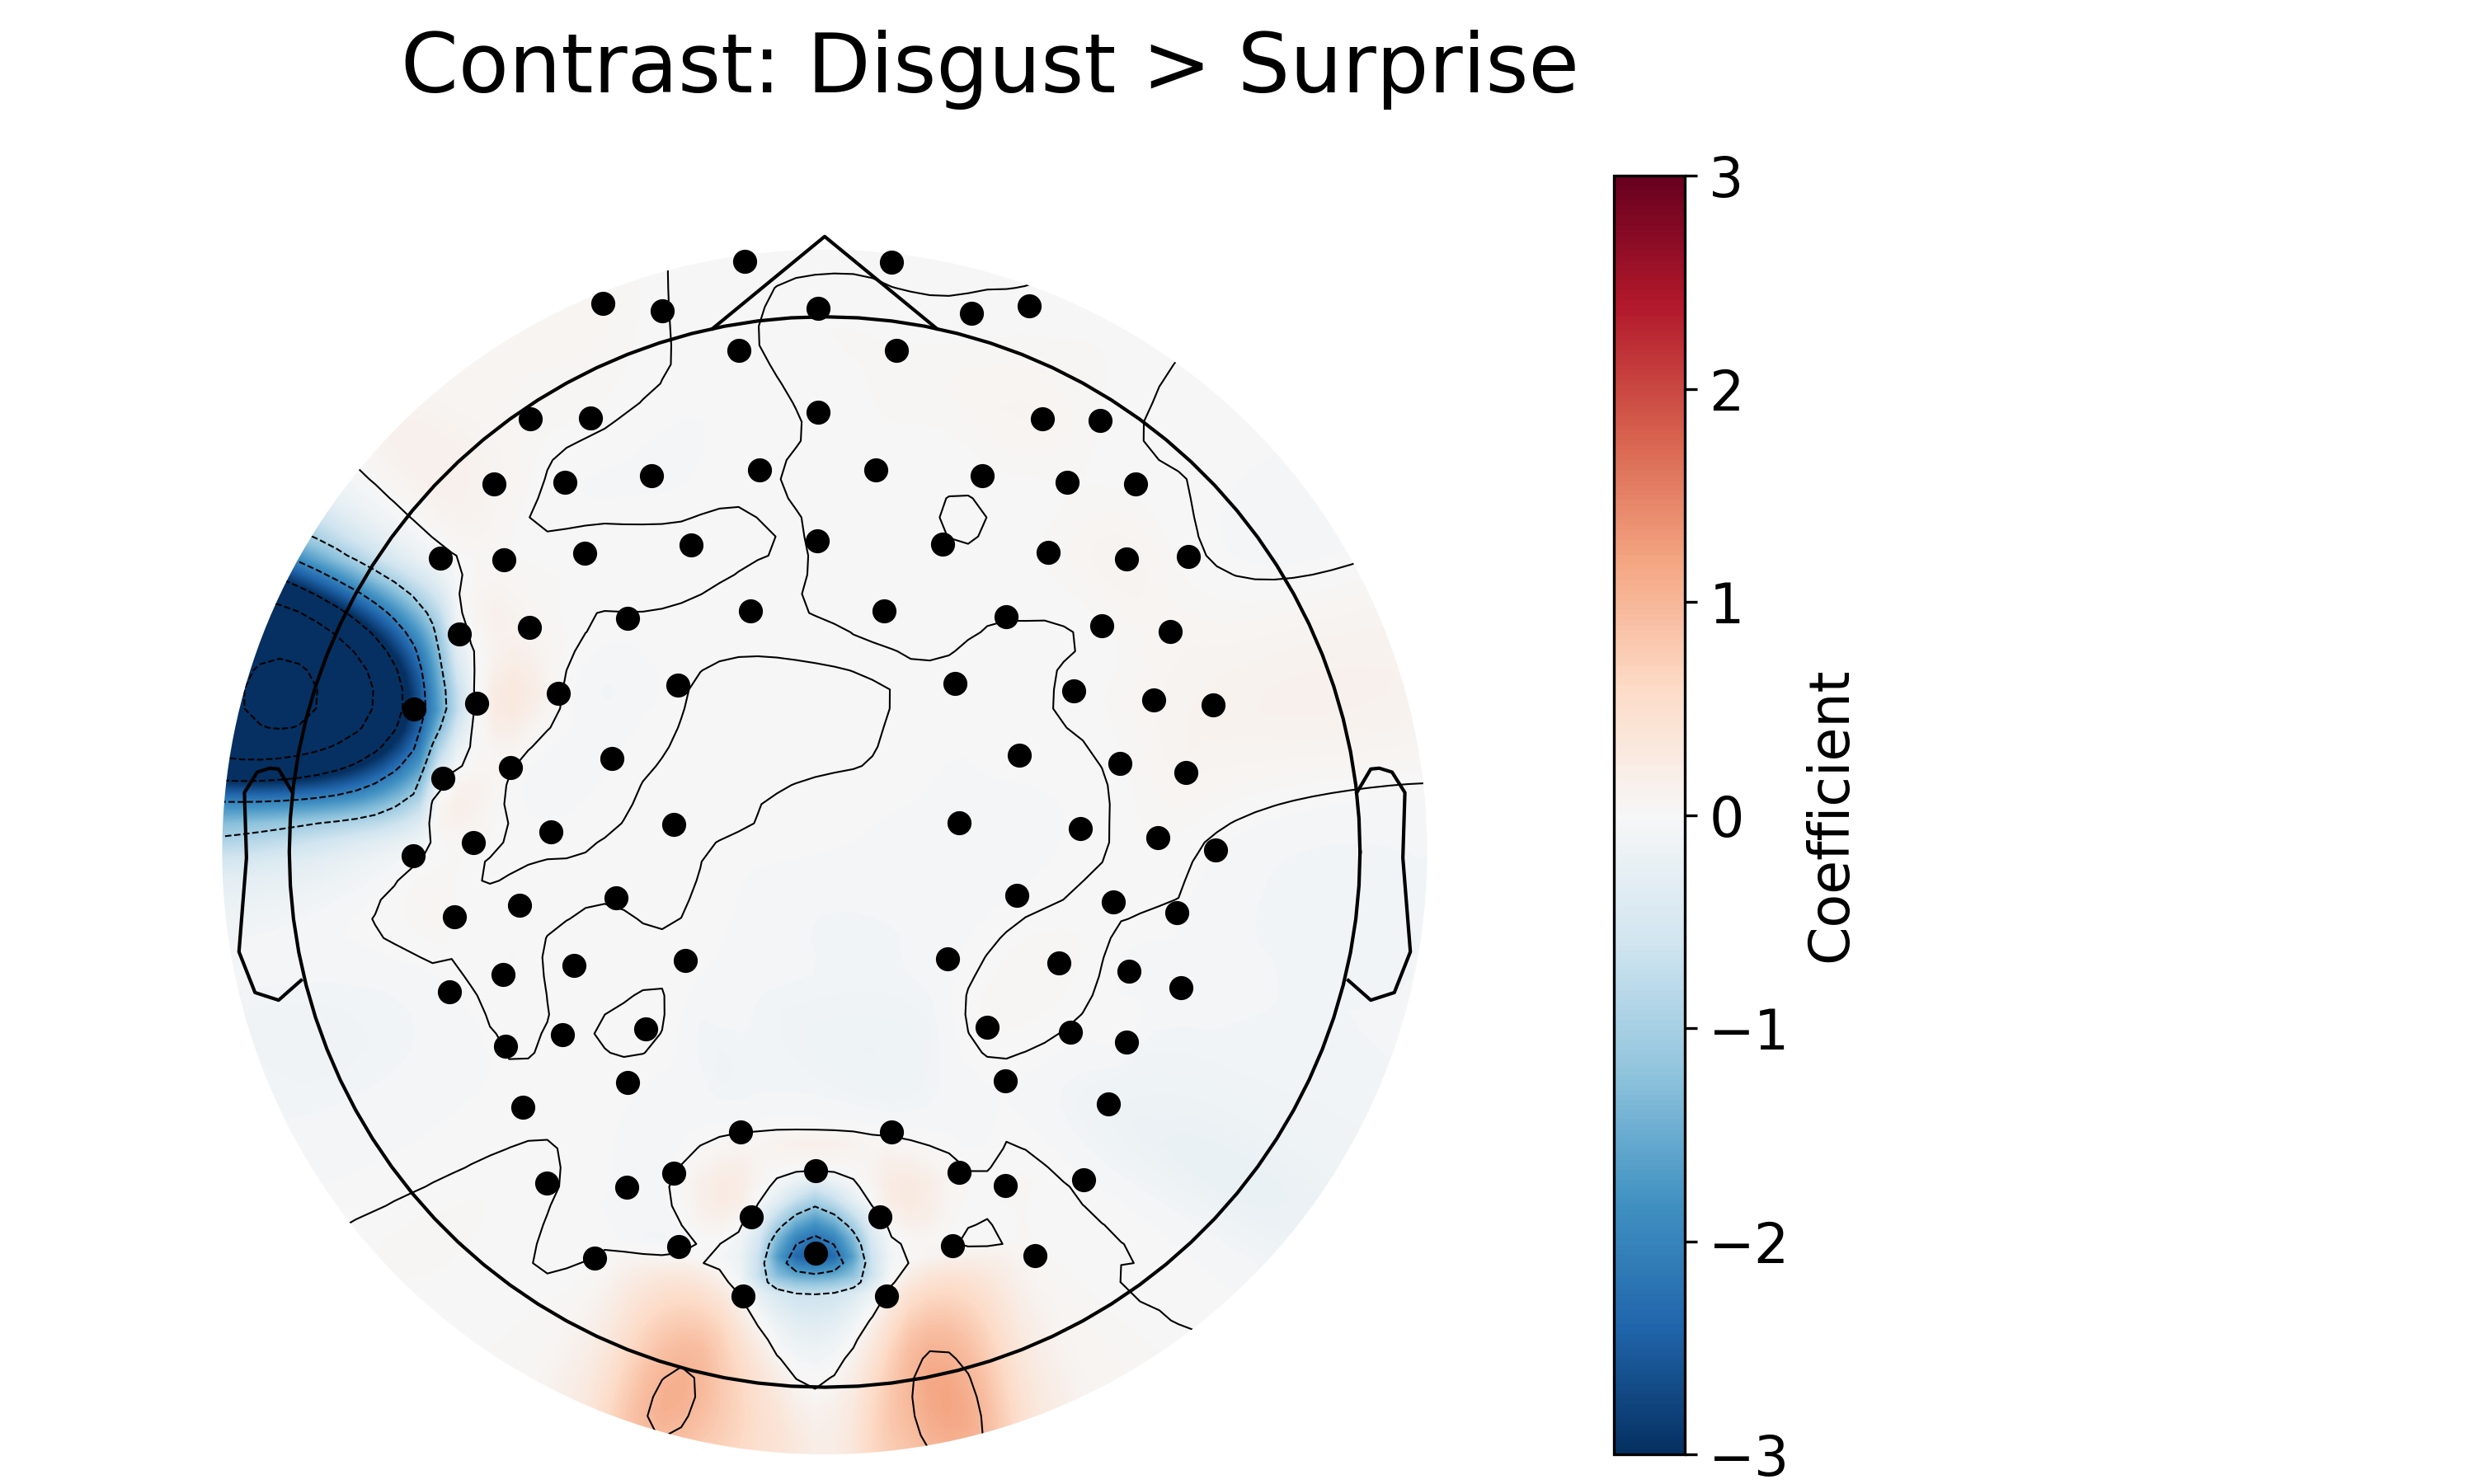
\includegraphics[width=0.29\textwidth, clip, trim=40 0 160 0]{C:/Users/super/OneDrive - Ontario Tech University/fNIRS_Emotions/plots/glm/contrasts/differences/Contrast_Disgust-Surprise.png} &
                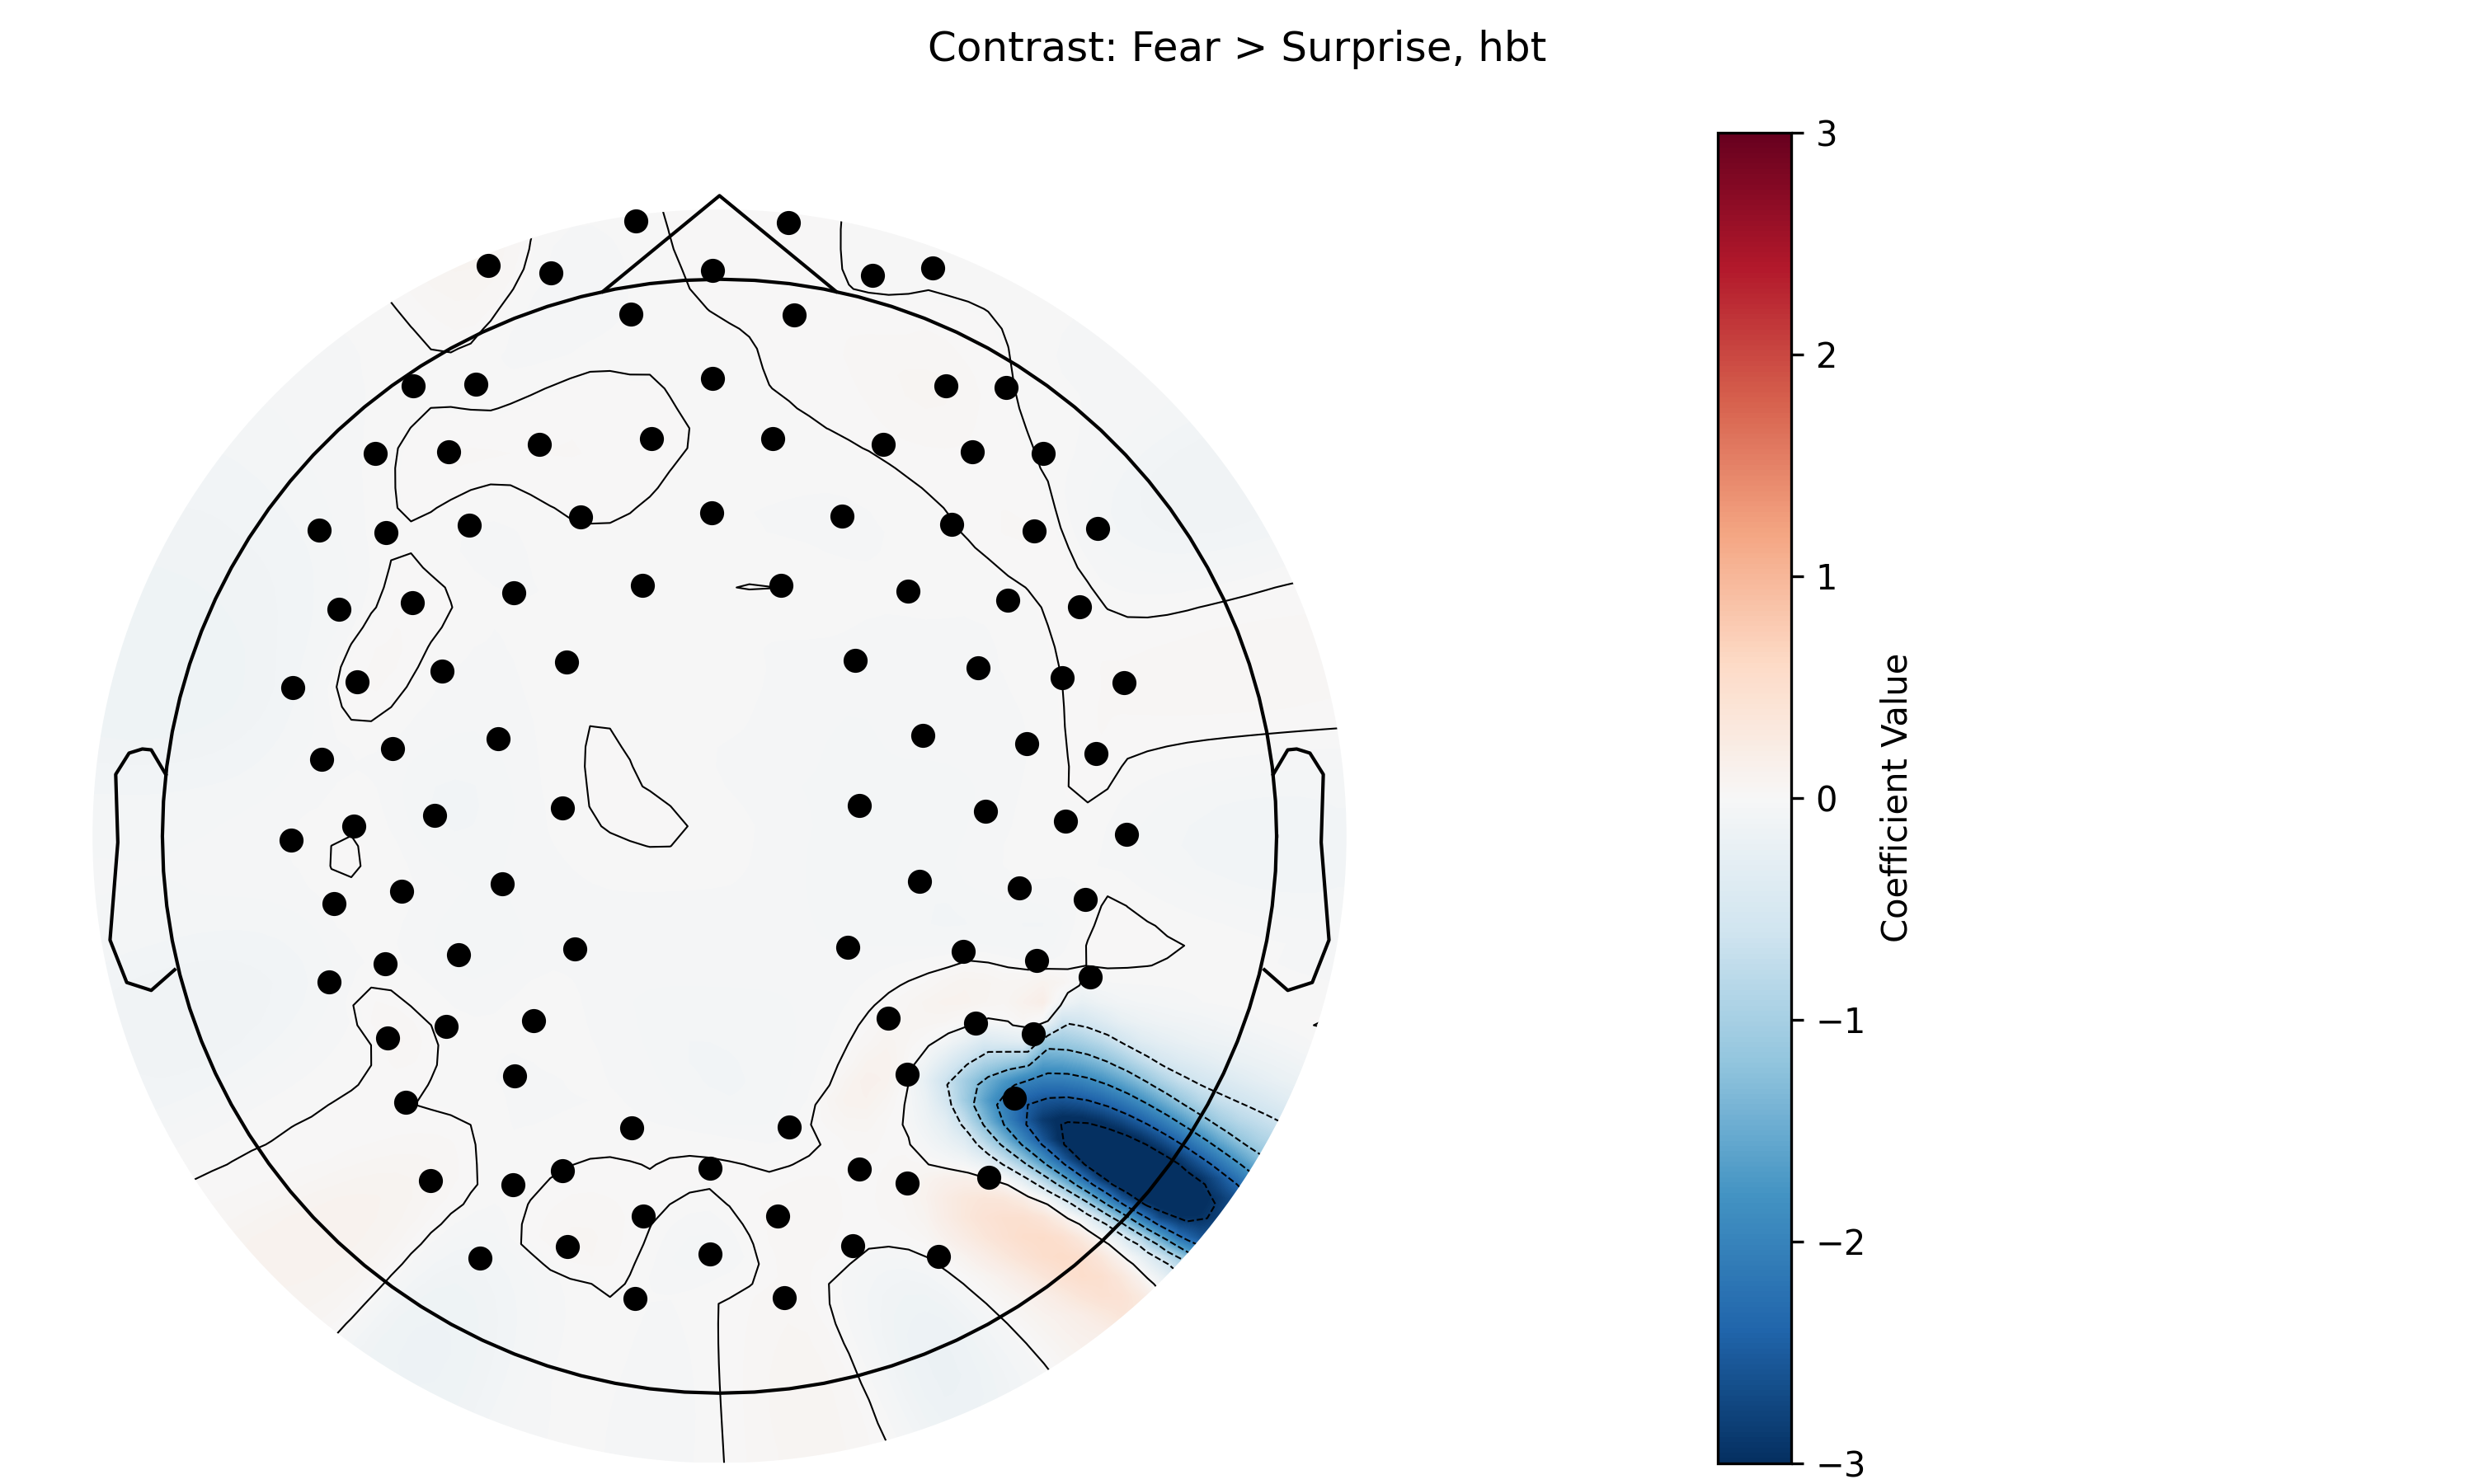
\includegraphics[width=0.29\textwidth, clip, trim=40 0 160 0]{C:/Users/super/OneDrive - Ontario Tech University/fNIRS_Emotions/plots/glm/contrasts/differences/Contrast_Fear-Surprise.png} \\
                
\includegraphics[width=0.29\textwidth, clip, trim=40 0 160 0]{C:/Users/super/OneDrive - Ontario Tech University/fNIRS_Emotions/plots/glm/contrasts/differences/Contrast_Joy-Surprise.png} &
                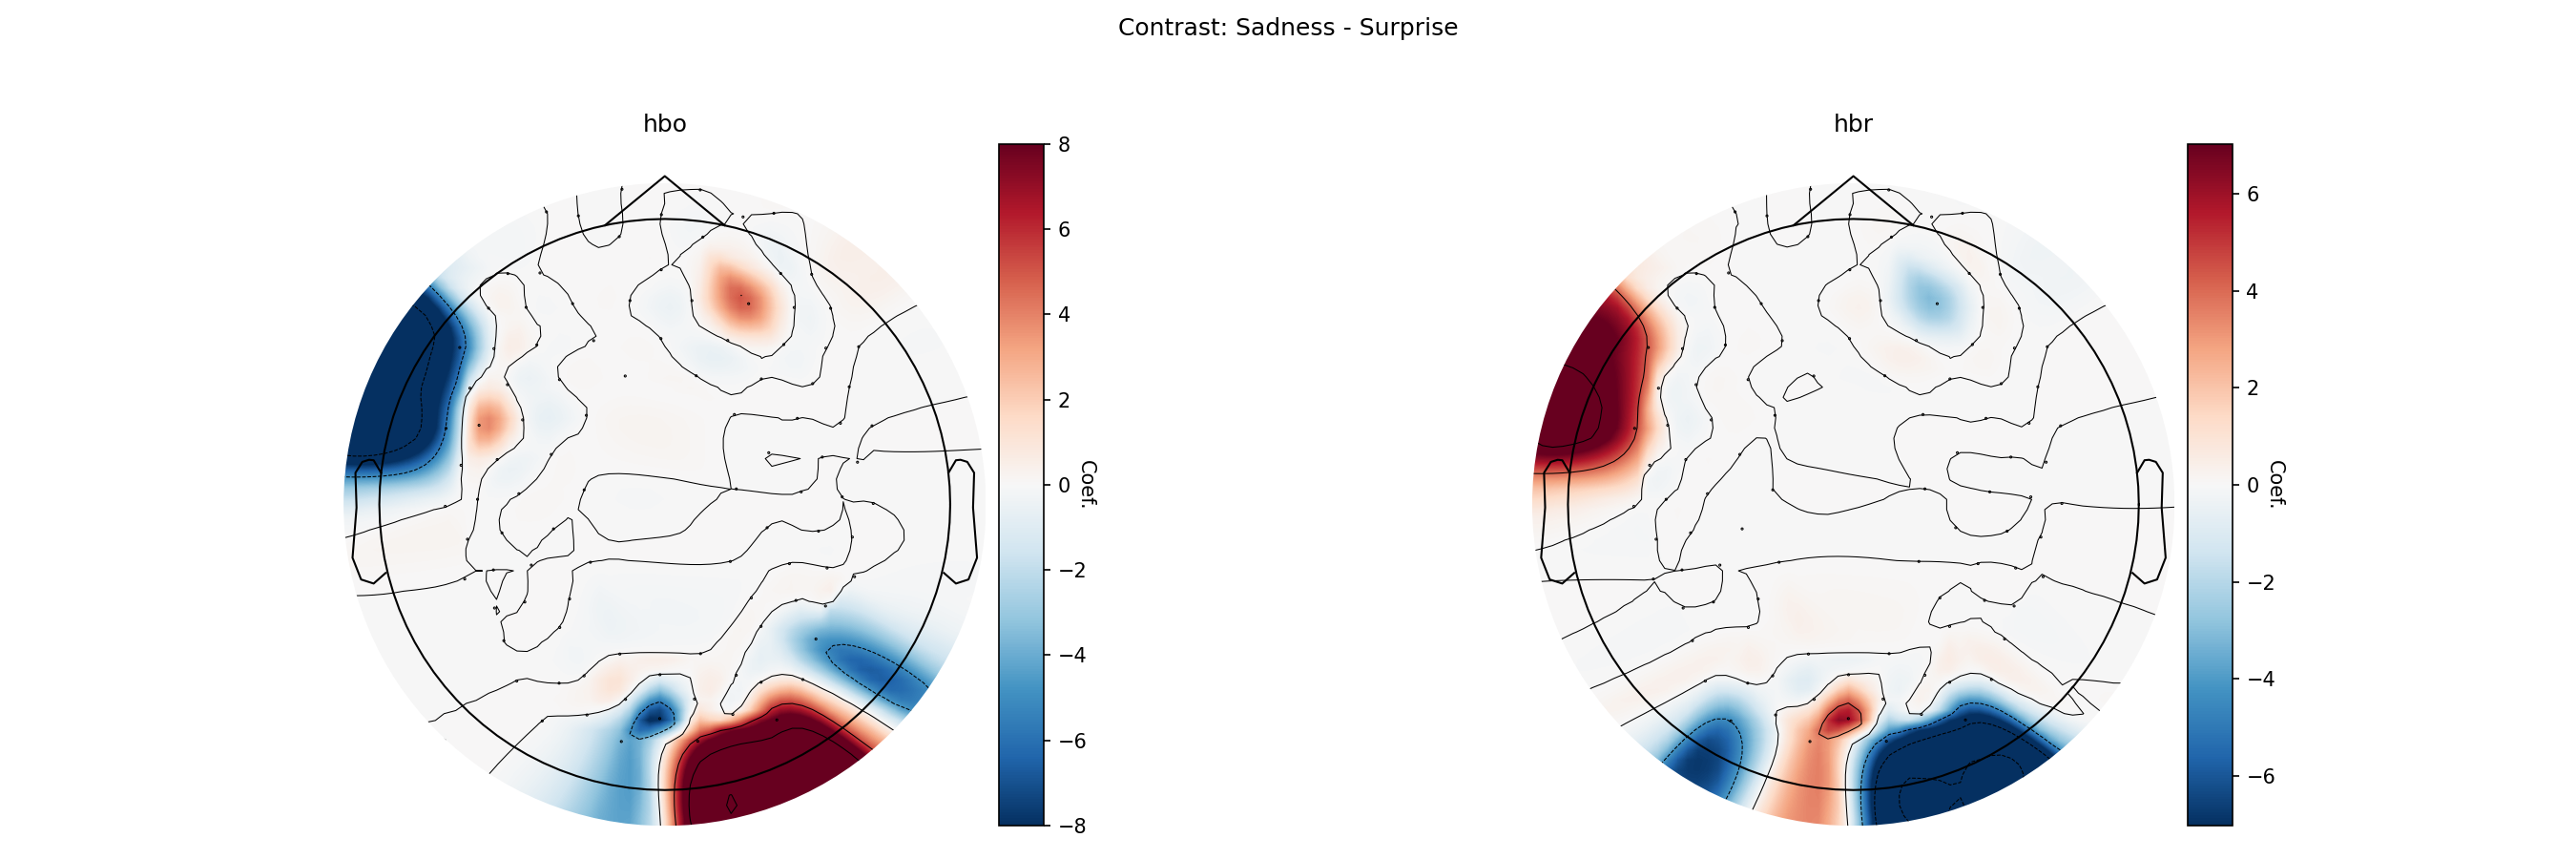
\includegraphics[width=0.29\textwidth, clip, trim=40 0 160 0]{C:/Users/super/OneDrive - Ontario Tech University/fNIRS_Emotions/plots/glm/contrasts/differences/Contrast_Sadness-Surprise.png} &
                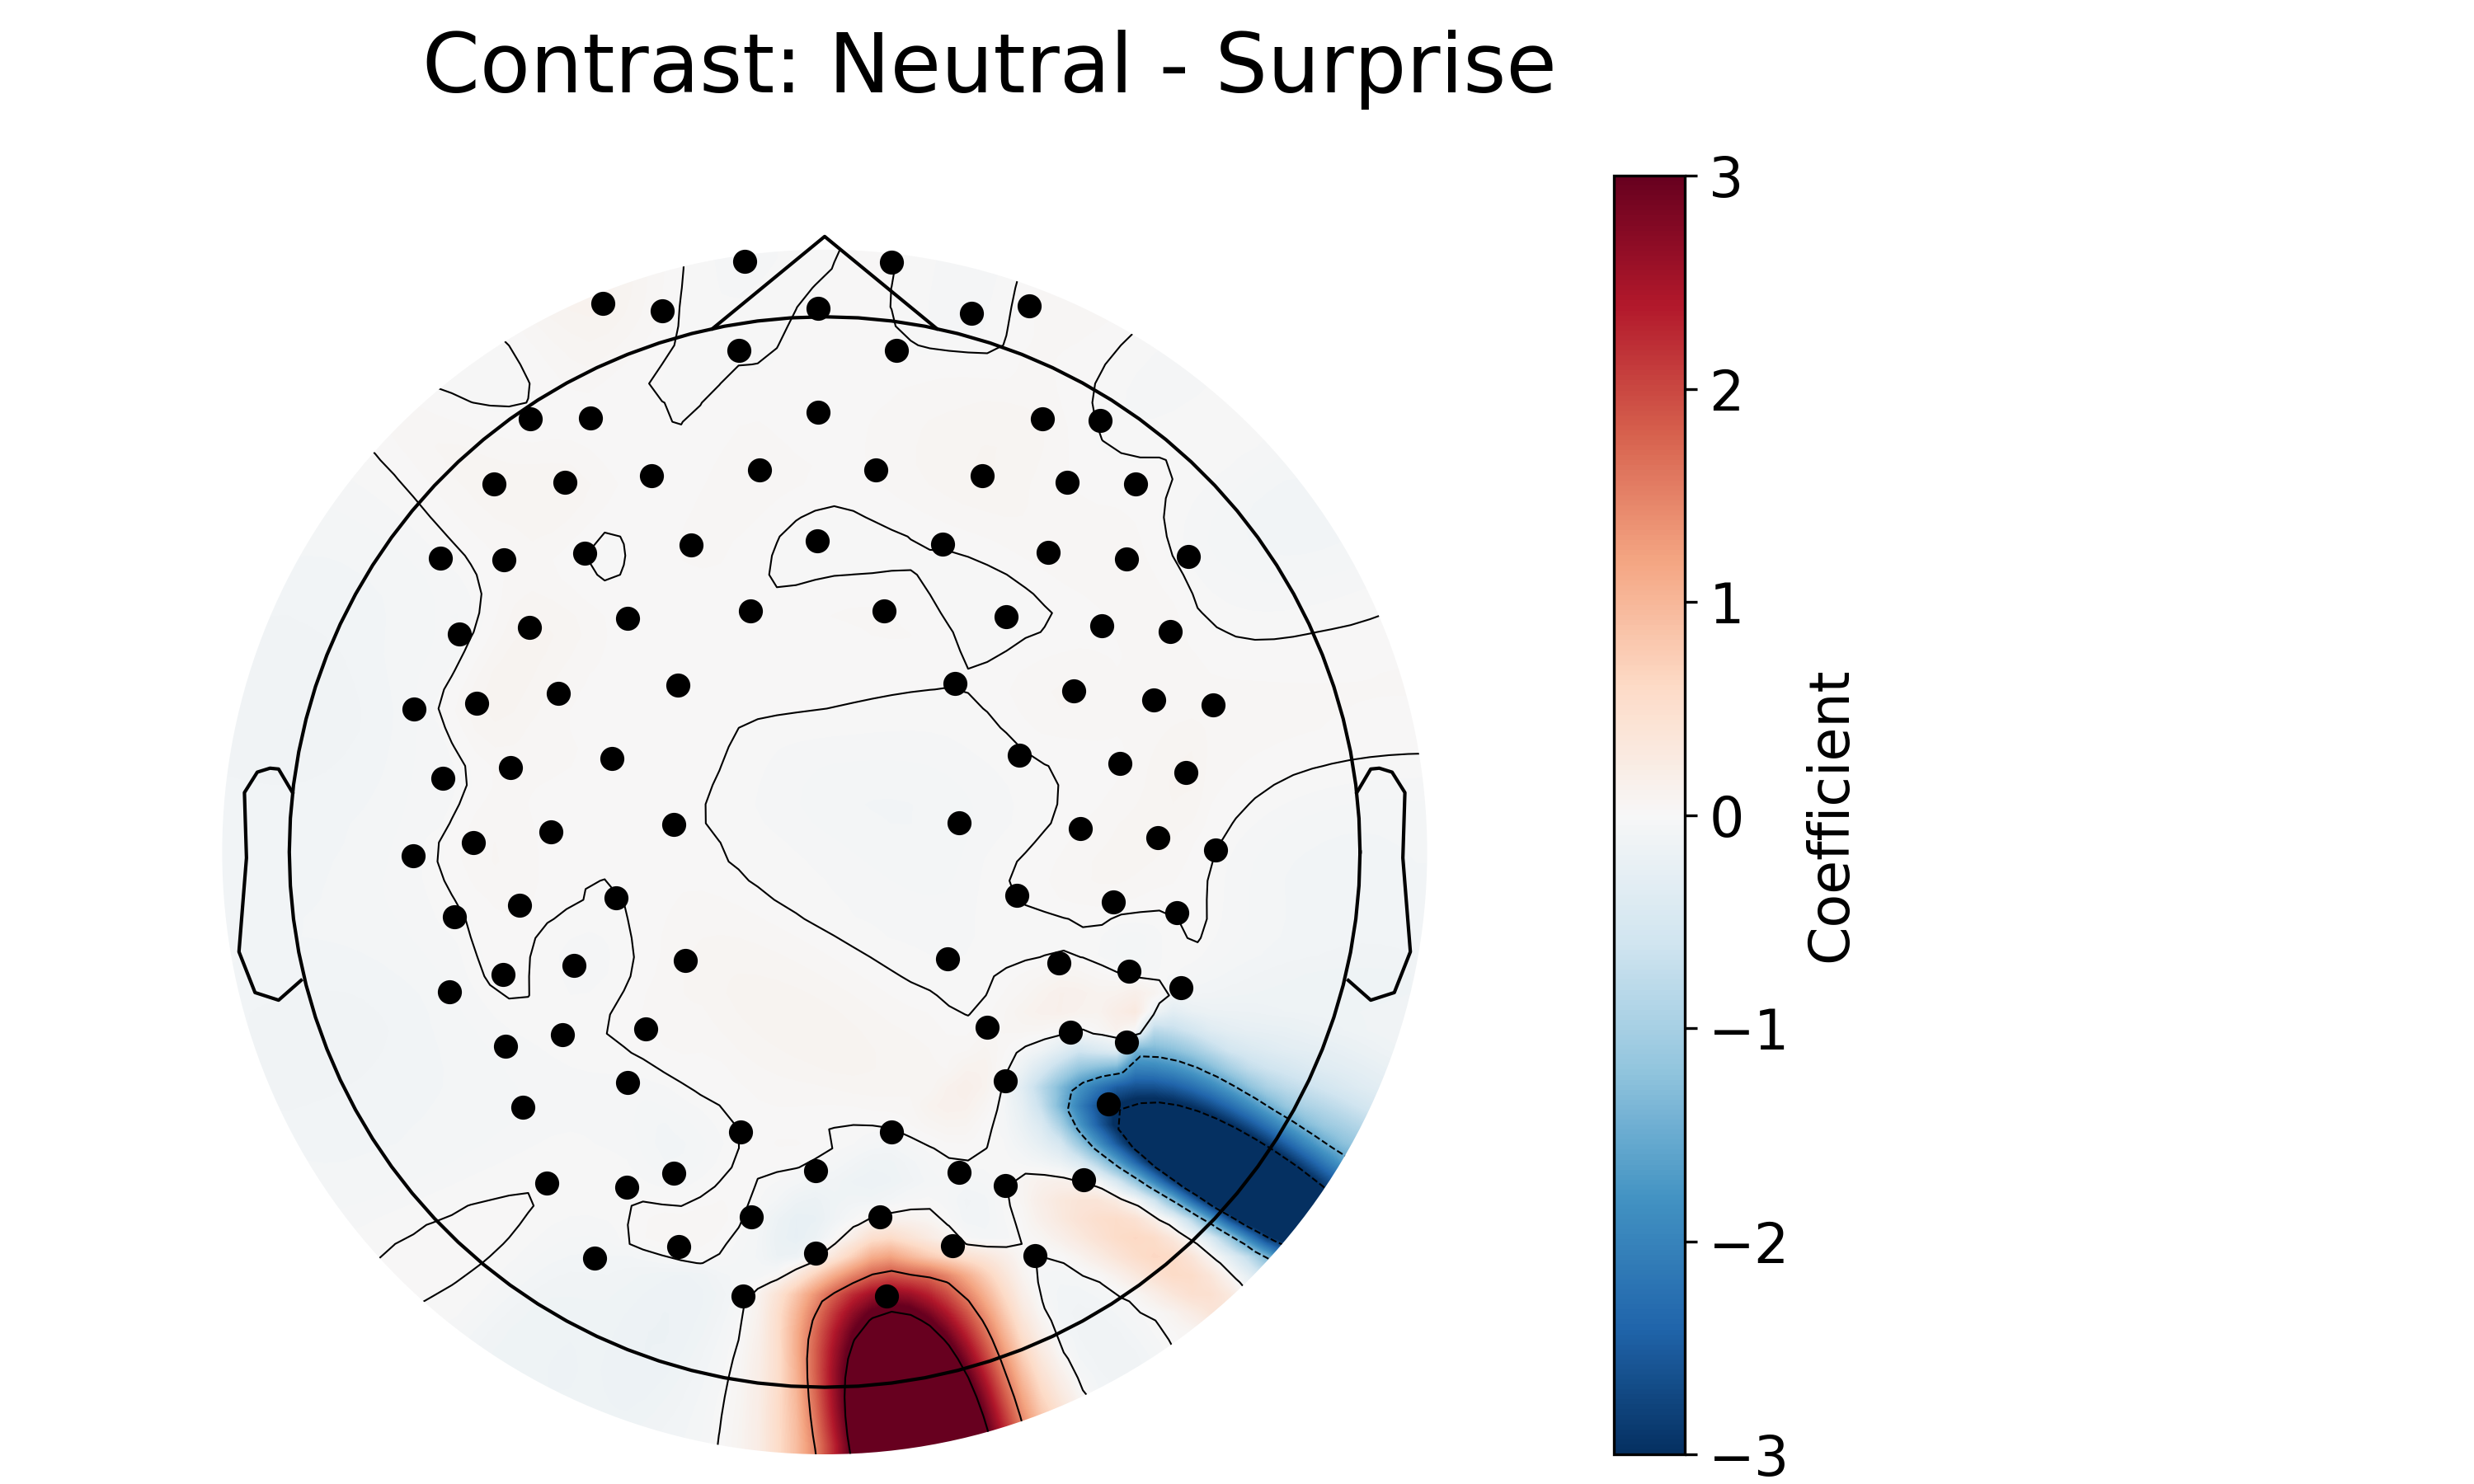
\includegraphics[width=0.29\textwidth, clip, trim=40 0 160 0]{C:/Users/super/OneDrive - Ontario Tech University/fNIRS_Emotions/plots/glm/contrasts/differences_neutral/Contrast_Neutral-Surprise.png} \\
            \end{tabular}
        \end{figure}
    \end{figure}
    \begin{itemize}
        \small
        \item Surprisingly, the GLM contrast for Surprise vs. all other emotions shows differences in activation in multiple regions. (except anger)
        \item \textbf{No other pairs of emotions showed significant differences.}
    \end{itemize}
    \note[frame]{
        \begin{itemize}
            \item Surprisingly, (pun intended) Surprise vs. all of the other emotions shows differences in activation in multiple regionsas well, except for anger.
            \item I'd like to note that these contrasts were run between all combinations of emotions, but only Surprise and Neutral showed significant differences, there were no other pairs of emotions (i.e. Joy-Sadness, Fear-Anger) that showed significant differences. 
        \end{itemize}
    }
\end{frame}

\begin{frame}
    \frametitle{Results}
    \framesubtitle{Emotional Faces}
    \begin{figure}
        \centering
        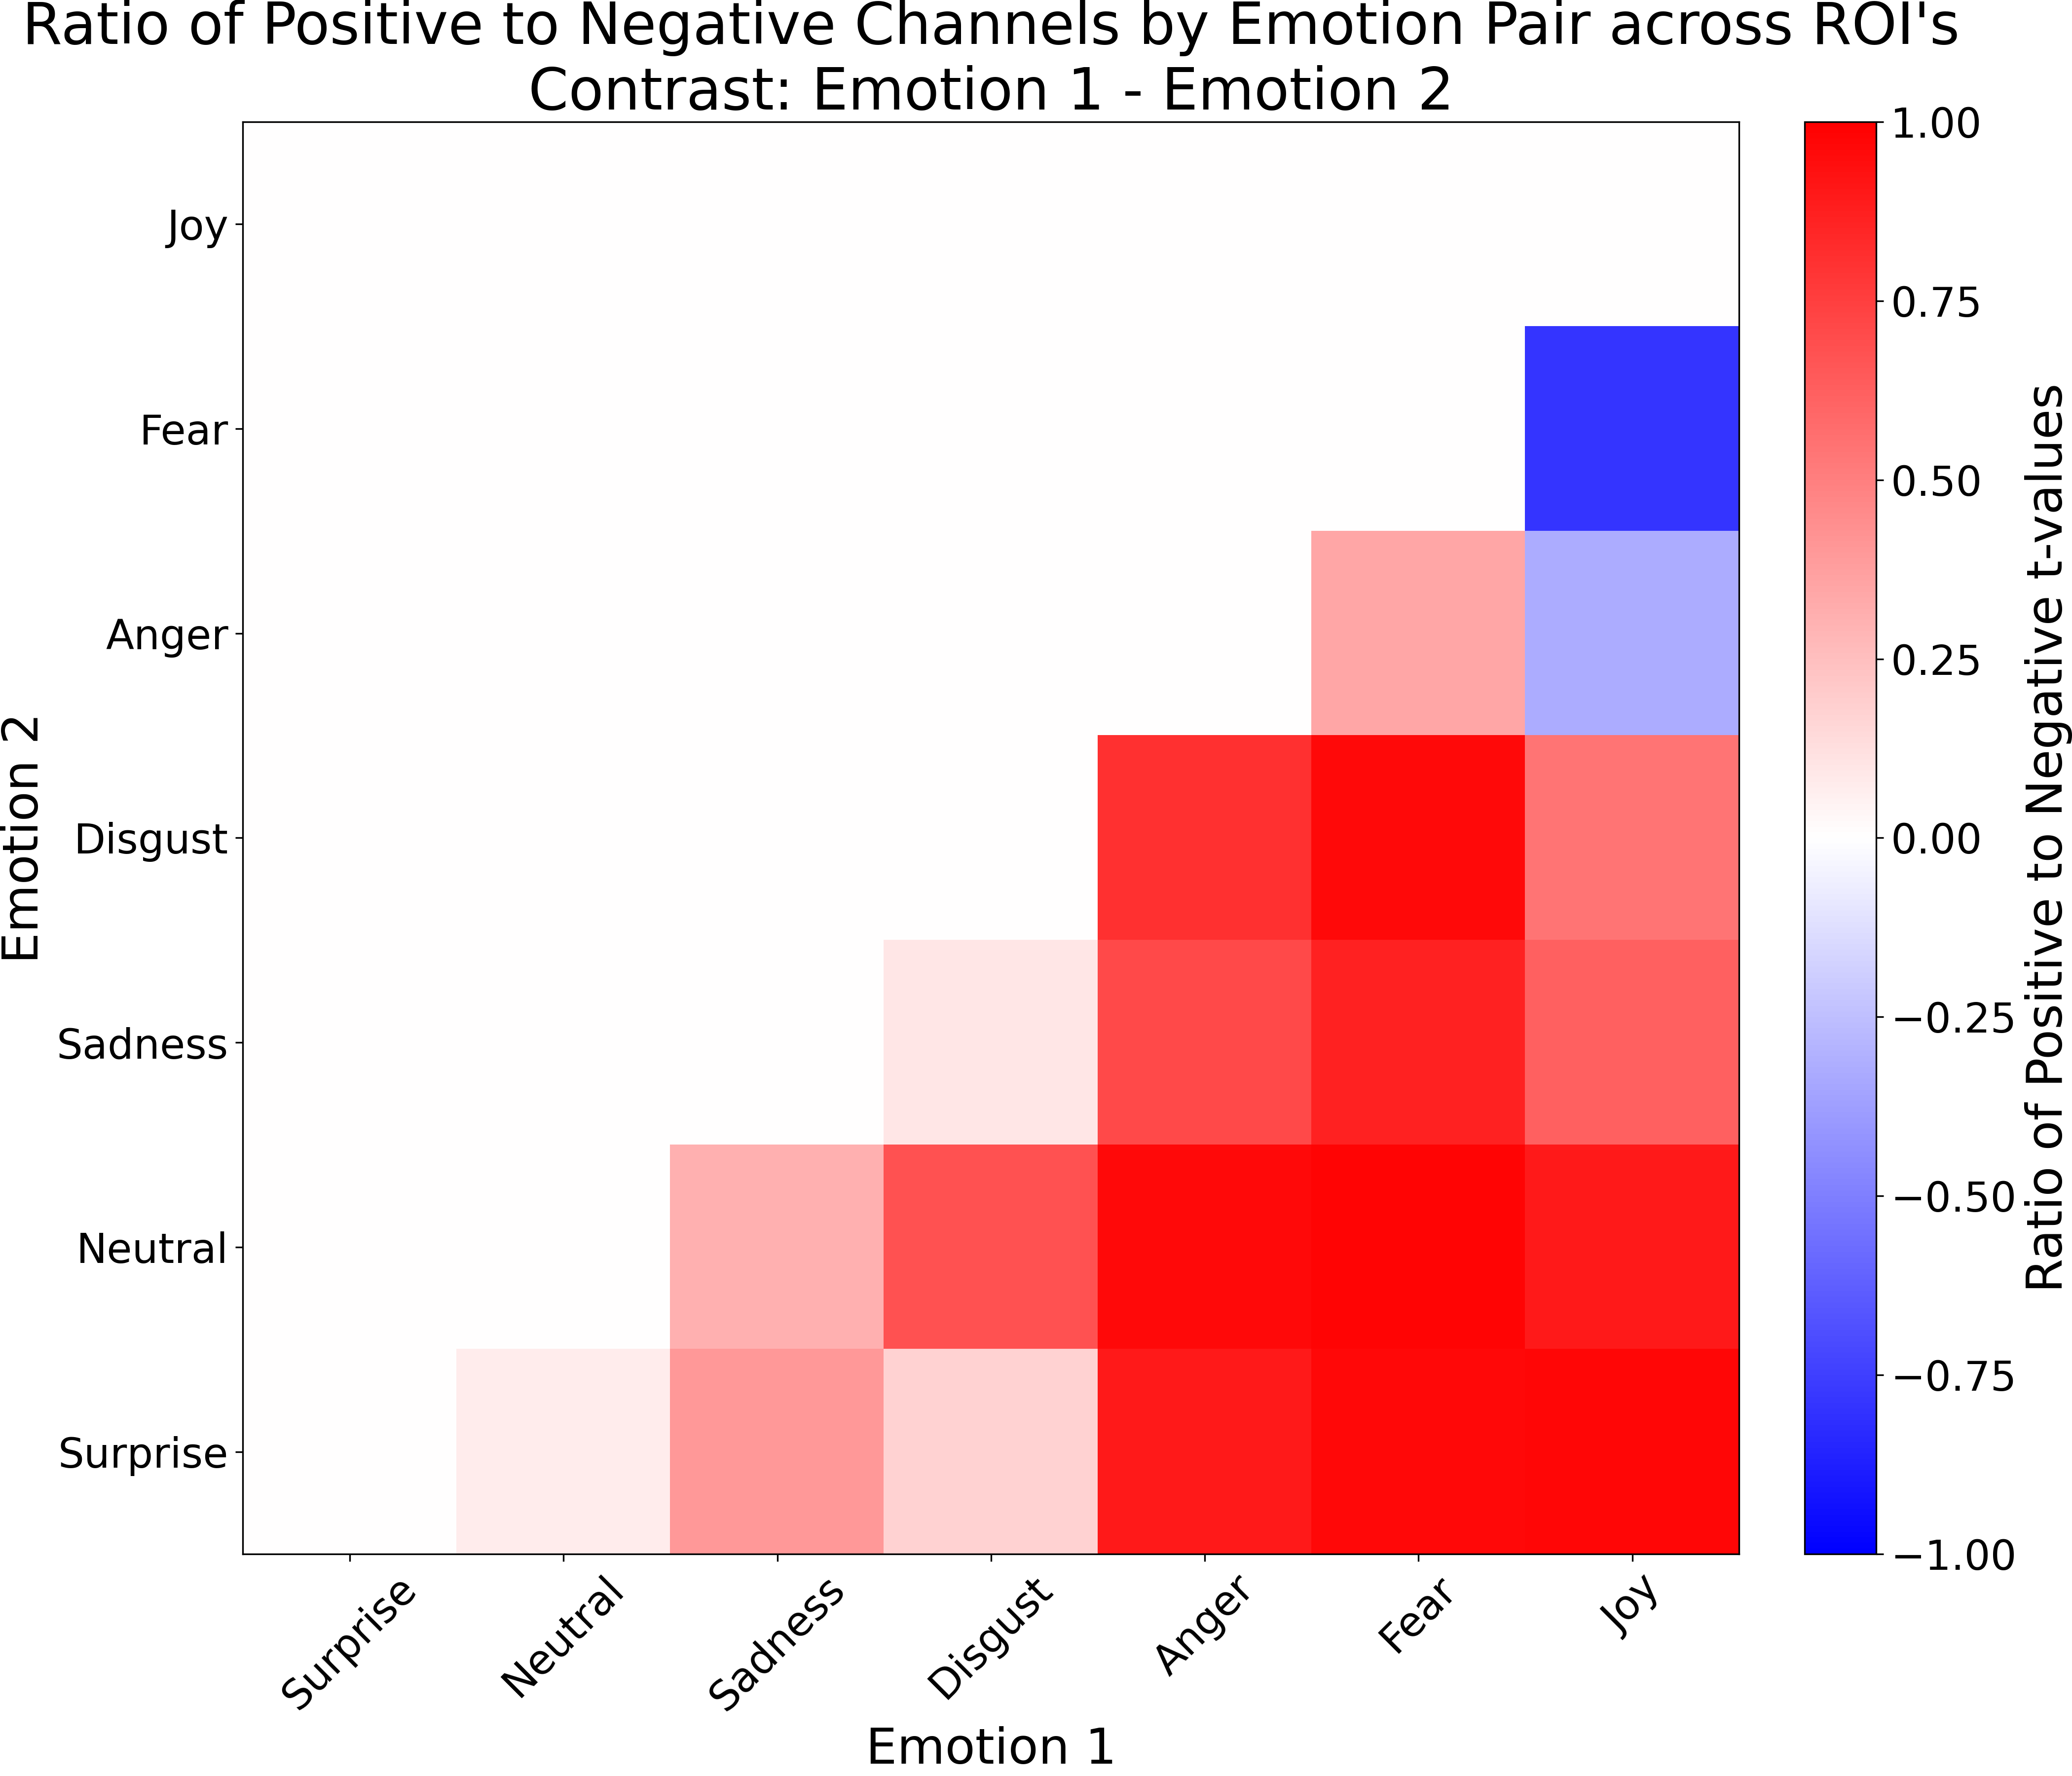
\includegraphics[width=0.7\textwidth]{C:/Users/super/OneDrive - Ontario Tech University/fNIRS_Emotions/plots/spectral_connectivity_time/emotion_analysis/emotion_contrast_heatmap.png}
    \end{figure}
    \begin{itemize}
        \small
        \item Count of significantly different channel pairs by emotion. 
        \item We see the largest differences in absolute connectivity levels for the Fear-Surprise pair, and more similarities in connectivity for the Joy-Anger pair.
    \end{itemize}
    \note[frame]{
        \begin{itemize}
            \item So we've seen the difference in activation in emotions, but we also wanted to look at the differences in connectivity for the emotional faces, this is a bit more of a complex story but there's some exciting results here.
            \item So here we have the count of significantly different channel pairs by emotion. 
            \item For example, we see that there are large differences in absolute levels of connectivity for Fear-Surprise pair, and more simllarities in connectivity for Joy-Anger pair.
            \item This is telling us that across all regions of the brain, the connectivity for the Fear-Surprise pair is more synchronized than the Joy-Anger pair. 
        \end{itemize}
    }
\end{frame}

\begin{frame}
    \frametitle{Results}
    \framesubtitle{Emotional Faces}
    \begin{figure}
        \centering
        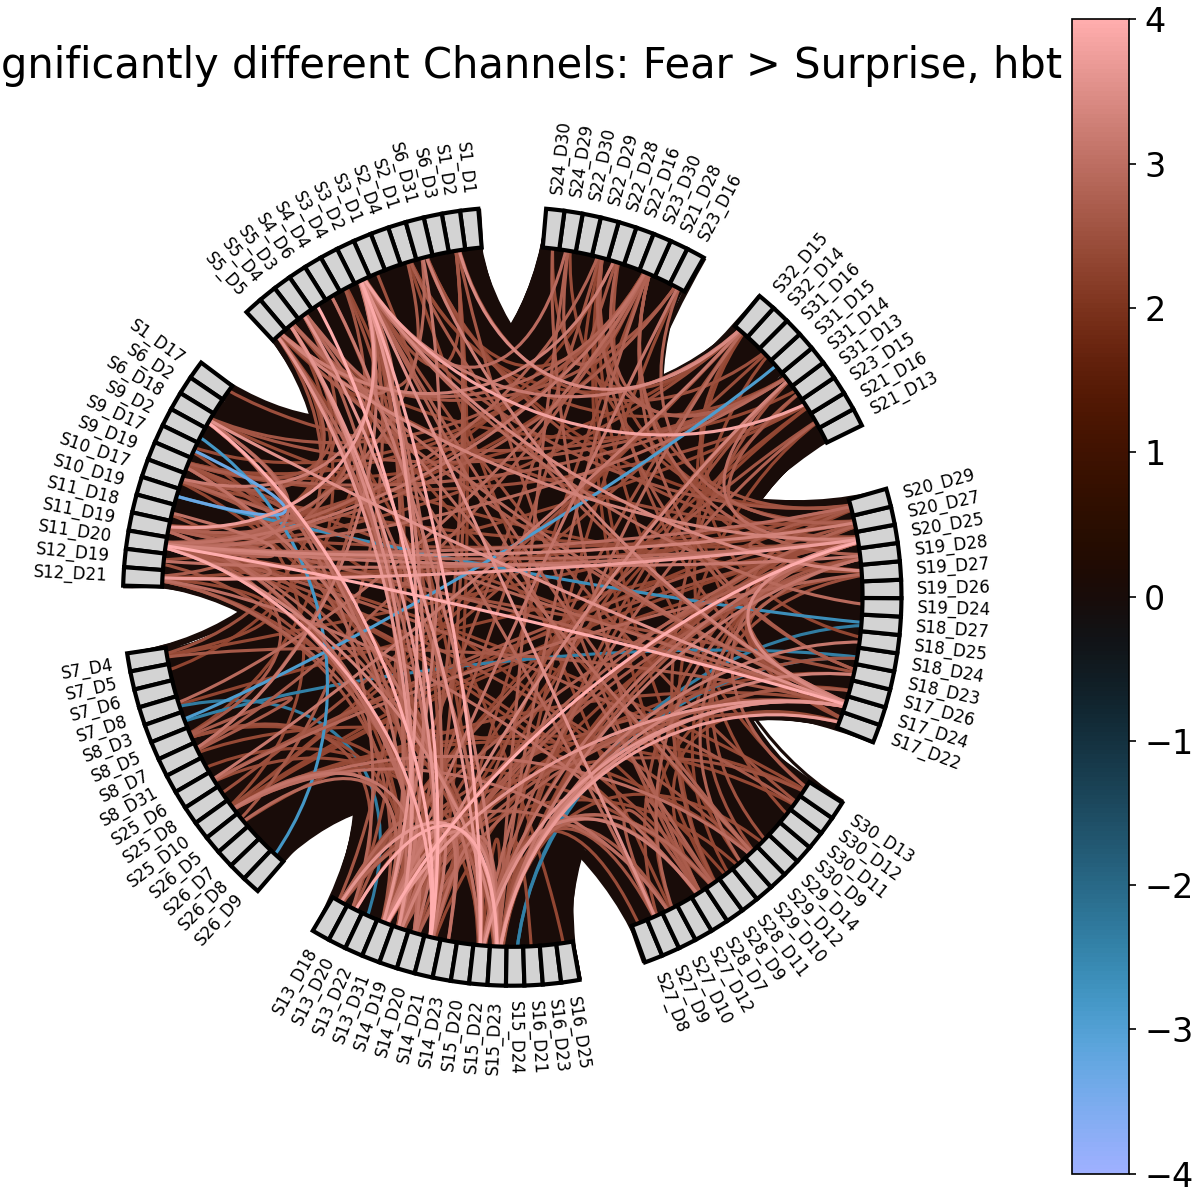
\includegraphics[width=0.49\textwidth]{C:/Users/super/OneDrive - Ontario Tech University/fNIRS_Emotions/plots/spectral_connectivity_time/chord_plots/group_level_t_tests_roi/emotion_Fear_Surprise.png}
        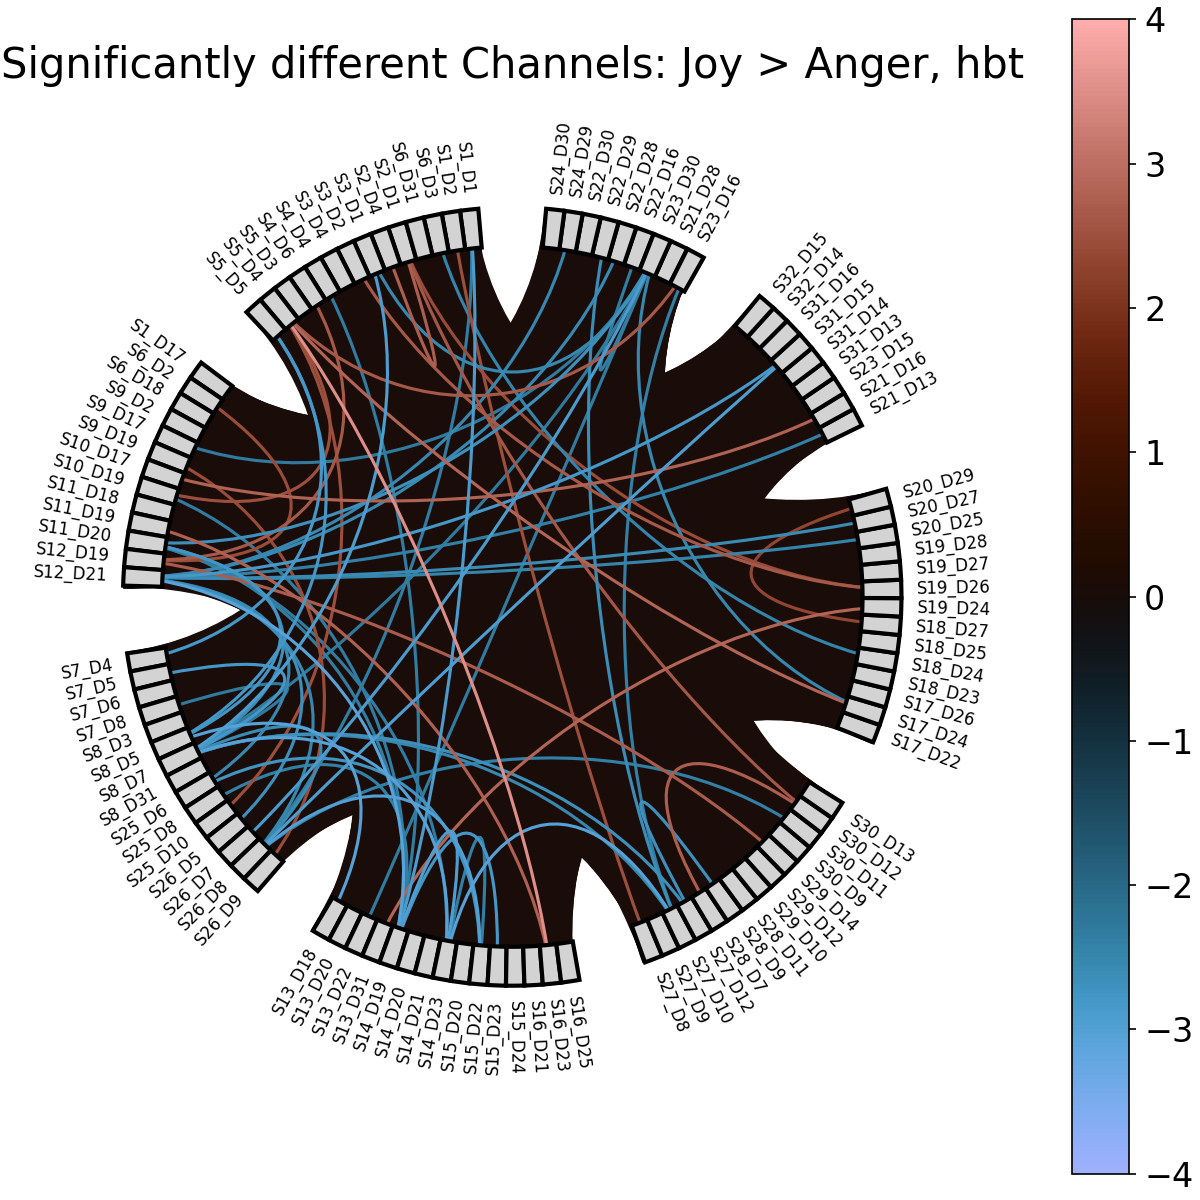
\includegraphics[width=0.49\textwidth]{C:/Users/super/OneDrive - Ontario Tech University/fNIRS_Emotions/plots/spectral_connectivity_time/chord_plots/group_level_t_tests_roi/emotion_Joy_Anger.png}
    \end{figure}
    \begin{itemize}
        \small
        \item Significant differences in connectivity between regions for Fear-Surprise (left) and Joy-Anger (right).
        \item Both pairs of emotions show less differences in the occipital regions (left occipital and right occipital) and between themselves (Left and left occipital and right and right occipital).
    \end{itemize}
    \note[frame]{
        \begin{itemize}
            \item Now if we look at the difference in connectivity between regions for the Fear-Surprise pair on the left, and the Joy-Anger pair on the right.
            \item We see that that both pairs of emotions show less differences in the occipital regions, that is between the left occipital and right occipital regions. 
            \item However, the Fear-Surprise pair has less synchronized activity than the Joy-Anger pair in general, which is shown by the scale on the right side of the figure.
        \end{itemize}
    }
\end{frame}

\begin{frame}
    \frametitle{Results}
    \framesubtitle{Emotional Faces}
    \begin{figure}
        \centering
        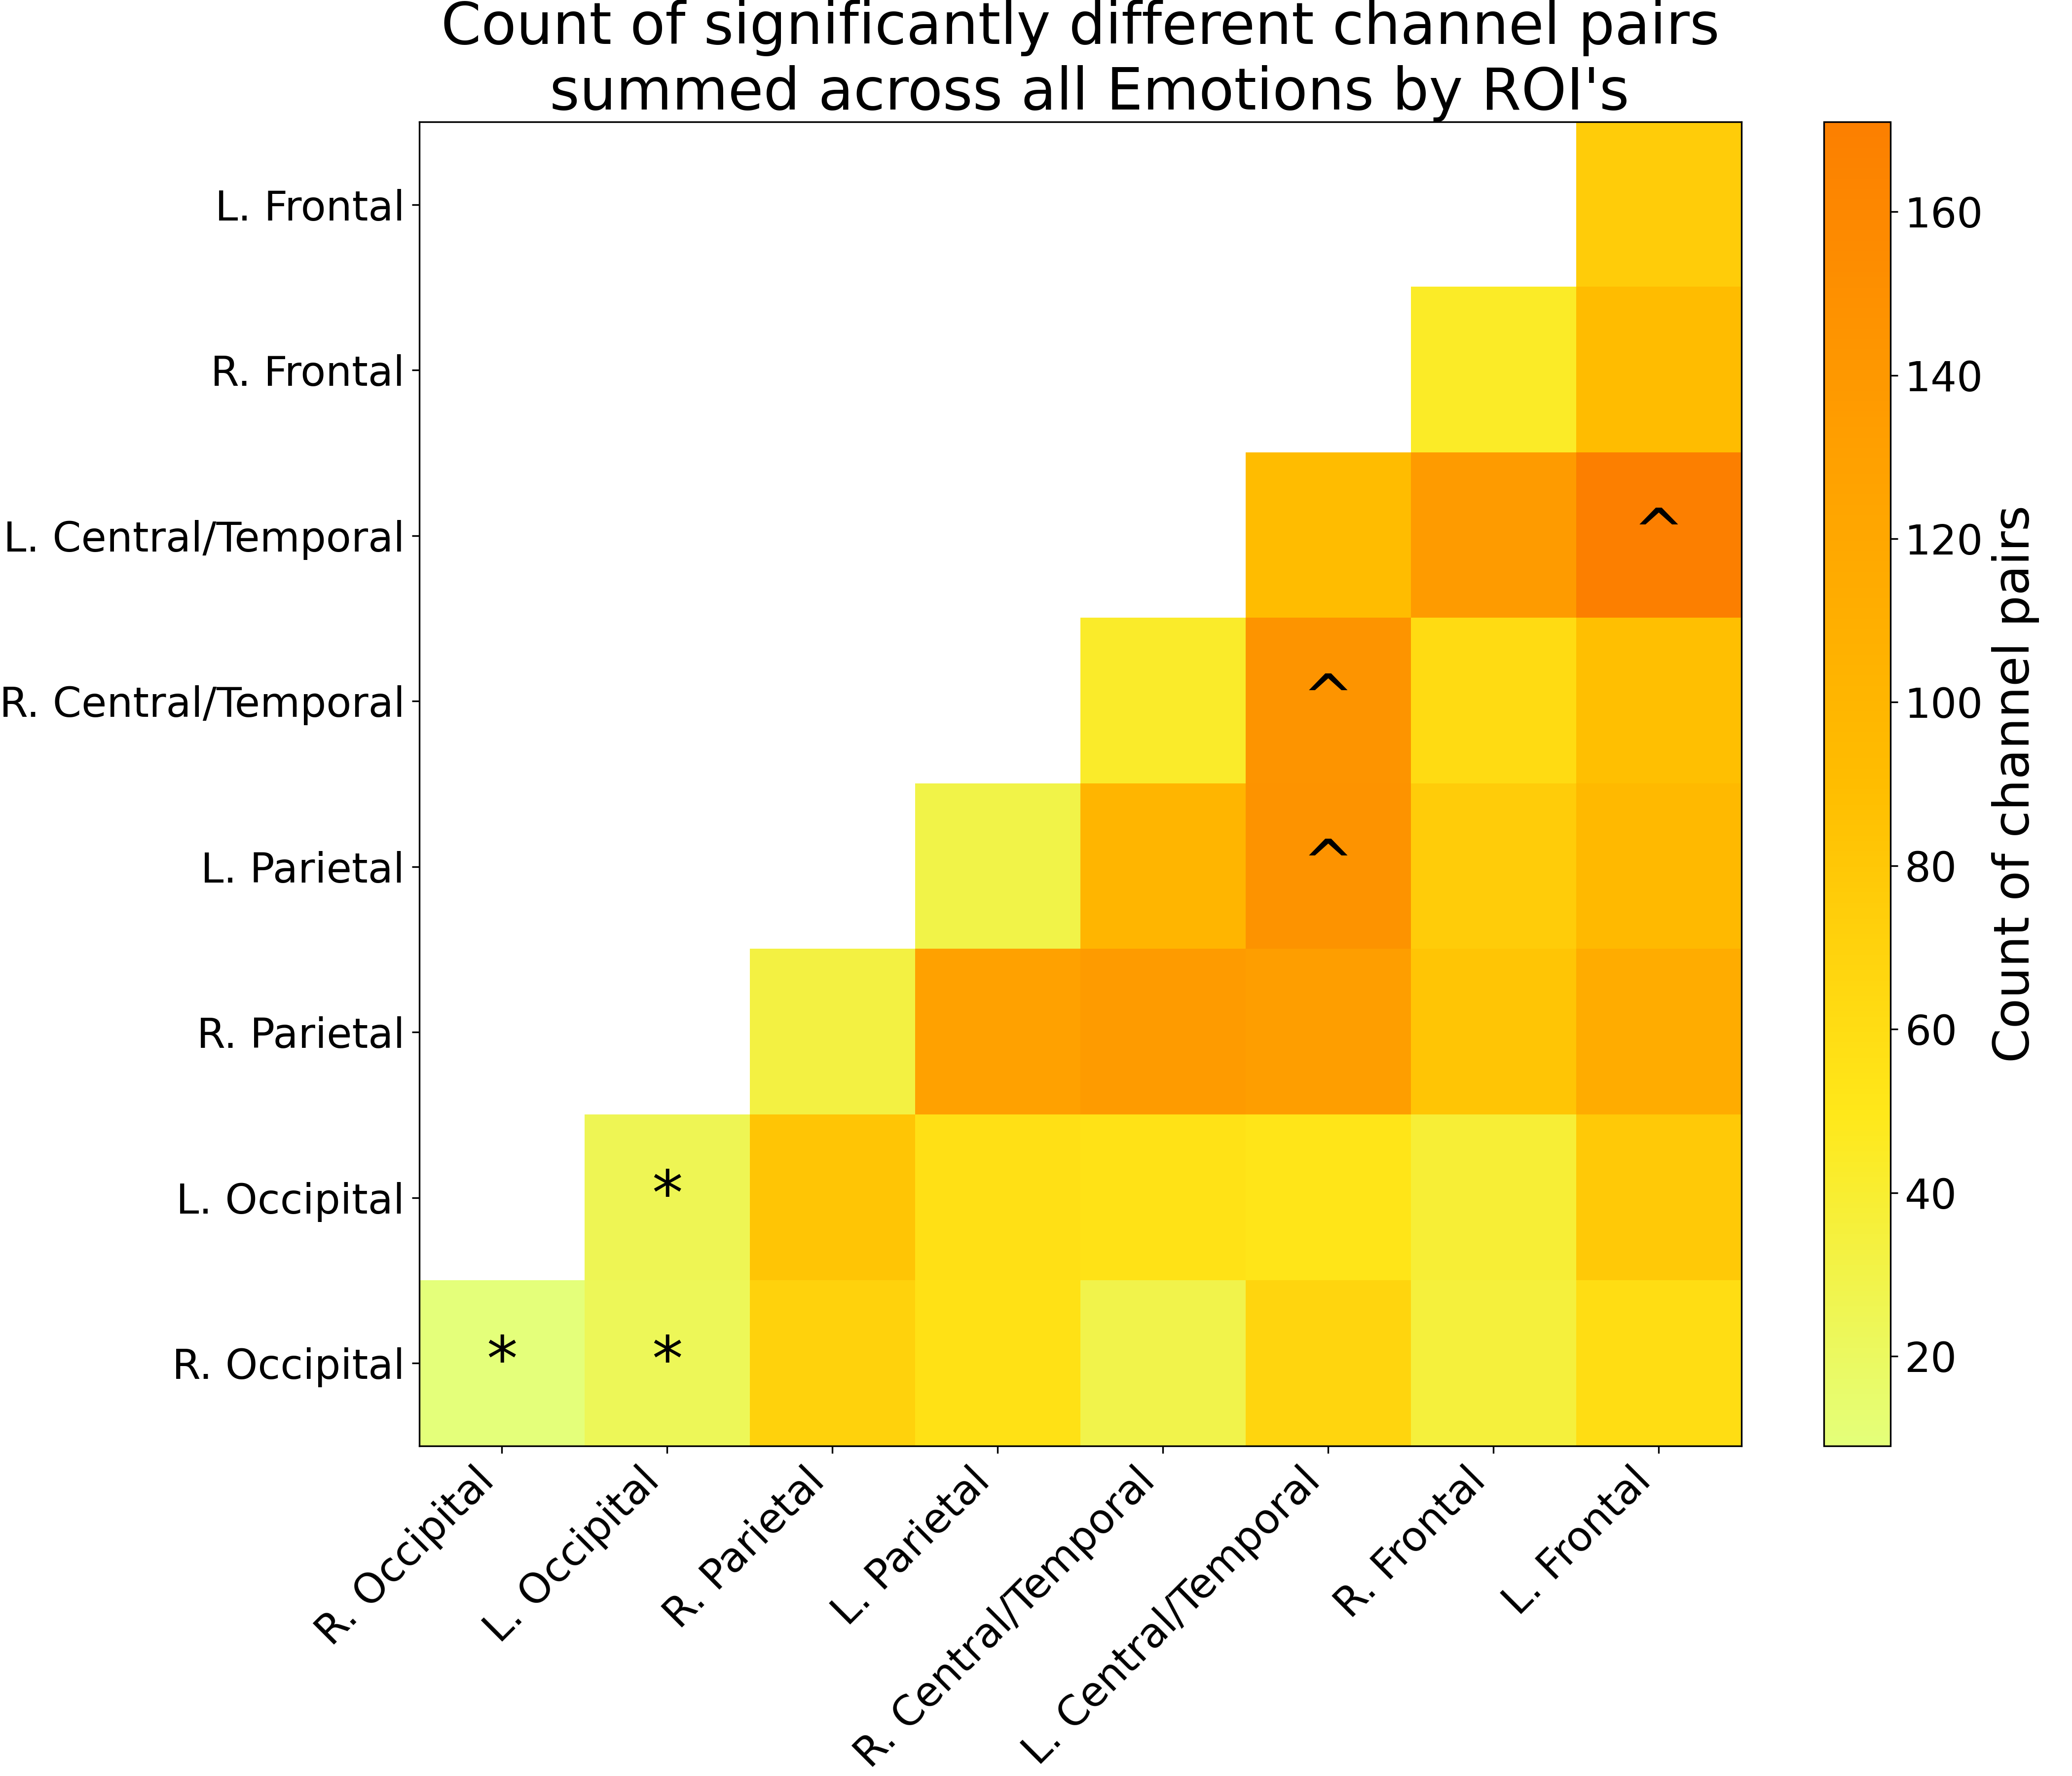
\includegraphics[width=0.75\textwidth]{C:/Users/super/OneDrive - Ontario Tech University/fNIRS_Emotions/plots/spectral_connectivity_time/emotion_analysis/region_contrast_heatmap.png}
    \end{figure}
    \begin{itemize}
        \small
        \item Count of significantly different channel pairs by region.
        \item The 3 regions with the most similarities in connectivity are marked with asterisks, which are all occipital regions.
    \end{itemize}
    \note[frame]{
        \begin{itemize}
            \item So here we have the count of significantly different channel pairs by region.
            \item The two figures I showed on the previous slide (if you remember) have the biggest difference in absolute connectivity levels, but have similar regional differences, especially in the occipital regions.
            \item I put asterisks on this figure, showing the 3 regions with the most similarities in connectivity, and it lines up with those two pairs of emotions shown on the previous slide.
            \item What this suggests is that the occipital regions are more synchronized with each other than any other pair of regions no matter the emotion, which is an incredibly interesting finding, I think. 
        \end{itemize}
    }
\end{frame}

\begin{frame}
    \frametitle{Discussion}
    \framesubtitle{Real vs. Virtual Faces}
    \textbf{Real vs. Virtual Faces:} 
    \begin{itemize}
        \small
        \item $H_1$: Differential activity between real and virtual faces. \\ 
        \begin{itemize}
            \item There is increased left occipital activation for virtual faces, compared to real faces. 
            \item There are significant differences in connectivity between:
            \begin{itemize}
                \item Left Frontal-Left Parietal regions
                \item Left Prefrontal-Right Occipital regions
            \end{itemize}
            \item These regions indicate real and virtual faces are processed differently—more so than GLM results suggest.
        \end{itemize}
    \end{itemize}
    \note[frame]{
        \begin{itemize}
            \item So what do these results mean? 
            \item The first thing we can take away from this is that virtual faces have increased activation in the left occipital region compared to real faces. 
            \item The connectivity differences between the left frontal and left parietal regions, and between the left prefrontal and right occipital regions indicate that real and virtual faces are processed differently, and more so than the GLM results suggest.
            \item So to answer our first hypothesis, we can say that there are indeed differences in brain activity between real and virtual faces, but these differences really come to light more in the connectivity results than in the GLM results.
        \end{itemize}
    }
\end{frame}

\begin{frame}
    \frametitle{Discussion}
    \framesubtitle{Emotional Faces}
    \textbf{Emotional Faces:}
    \begin{itemize}
        \small
        \item $H_2$: Differential activity across different emotions (anger, disgust, fear, happiness, sadness, surprise, neutral). \\ 
        \begin{itemize}
            \item Surprise and Neutral show higher activation in multiple regions compared to all other emotions. 
            \item The other emotions did not show significant differences in activation between each other. 
            \item Left occipital and right occipital regions show the most similarities in connectivity, suggesting they are more synchronized with each other than any other pair of regions, regardless of the emotion.
        \end{itemize}
    \end{itemize}
    \note[frame]{
        \begin{itemize}
            \item The second thing we can take away from this is that the emotional faces show significant differences in activation in multiple regions, but only for the Surprise and Neutral emotions.
            \item The other emotions did not show significant differences in activation, surprisingly.
            \item The left occipital and right occipital regions show the most similarities in connectivity, suggesting they are more synchronized with each other than any other pair of regions, regardless of the emotion.
            \item So to answer our second hypothesis, we can say that there are indeed differences in activation across emotions, and the occipital regions of the brain are more synchronized with each other across all emotions. 
        \end{itemize}
    }
\end{frame}

\begin{frame}
    \frametitle{Conclusion}
    \begin{itemize}
        \small        
        \item \textbf{Implications:}
        \begin{itemize}
            \item Offers insight into how the brain responds to virtual stimuli, relevant for Virtual Reality (VR), Brain Computer Interfaces (BCI).
            \item Can inform the design of more realistic and effective virtual characters in education and/or gaming. 
        \end{itemize}
        \item \textbf{Future Research:}
        \begin{itemize}
            \item Future research could explore how these neural differences influence real-world behaviors, or how they affect interactions in digital environments.
        \end{itemize}
    \end{itemize}
    \note[frame]{
        \begin{itemize}
            \item So in conclusion, this research offers insight into how the brain responds to virtual stimuli, which is relevant for applications in Virtual Reality (VR) like gaming or education. 
            \item As well as Brain Computer Interfaces (BCI), for example you can imagine having an fNIRS cap on, and using it to control a computer or a virtual character in a game.
            \item This research can inform the design of more realistic and effective virtual characters in education and/or gaming, which can help improve the user experience.
            \item Finally, future research could explore how these neural differences influence real-world behaviors, or how they affect interactions in digital environments.
            \item For example, we could look at how people react to virtual faces in video games, or how students might learn things differently when interacting with virtual teachers or avatars.
            \item Thank you for your time and attention. 
        \end{itemize}
    }
\end{frame}

\begin{frame}[allowframebreaks]
    \frametitle{References}
    \footnotesize
    \bibliographystyle{plainnat}
    \bibliography{references}
\end{frame}

\end{document}